%%%%%%%%%%%%%%%%%%%%%%%%%%%%%%%%%%%%%%%%%%%%%%%%%%%%%%%%%%%%
%%  This Beamer template was created by Matteo Rucco..
%%  Anyone can freely use or modify it for any purpose
%%  without attribution.
%%
%%  Last Modified: December 7, 2014
%%

\documentclass[xcolor=x11names,compress]{beamer}

%% General document %%%%%%%%%%%%%%%%%%%%%%%%%%%%%%%%%%
\usepackage{graphicx}
\usepackage{tikz}
\usepackage[inkscapeformat=png]{svg}
\usetikzlibrary{decorations.fractals}
\usepackage{listings}
\usepackage{wrapfig}
\usepackage{subcaption}

%%%%%%%%%%%%%%%%%%%%%%%%%%%%%%%%%%%%%%%%%%%%%%%%%%%%%%
% Configs

\graphicspath{{../tesi/Immagini}}

\lstdefinestyle{glydric}{
    columns=fullflexible,
    basicstyle=\small\ttfamily\fontfamily{pcr}\selectfont,
    numberstyle=\tiny\color{codegray},
    numbers=left,
    numbersep=2pt
}
\lstset{
    style=glydric,
    breaklines=true,
}

%% Beamer Layout %%%%%%%%%%%%%%%%%%%%%%%%%%%%%%%%%%
\useoutertheme[subsection=false,shadow]{miniframes}
\useinnertheme{default}
\usefonttheme{serif}
\usepackage{palatino}
\usepackage{setspace,textcomp,soul}

\setbeamerfont{title like}{shape=\scshape}
\setbeamerfont{frametitle}{shape=\scshape}
\definecolor{bluUnicam}{RGB}{27,43,74}
\definecolor{redUnicam}{RGB}{219,0,36}
\definecolor{orangeUnicam}{RGB}{234,114,40}
\setbeamercolor*{lower separation line head}{bg=redUnicam} 
\setbeamercolor*{normal text}{fg=bluUnicam,bg=white} 
\setbeamercolor*{alerted text}{fg=red} 
\setbeamercolor*{example text}{fg=black} 
\setbeamercolor*{structure}{fg=orangeUnicam} 
\setbeamercolor*{frametitle}{fg=redUnicam}

\setbeamercolor*{palette tertiary}{fg=orangeUnicam,bg=bluUnicam} 
\setbeamercolor*{palette quaternary}{fg=black,bg=black!10} 

\theoremstyle{definition} \newtheorem{esempio}{Esempio}
\theoremstyle{definition}
\newtheorem{definizione}{Definition} \theoremstyle{plain}
\newtheorem{teorema}{Theorem}

%%%%%%%%%%%%%%%%%%%%%%%%%%%%%%%%%%%%%%%%%%%%%%%%%%

\begin{document}

%%%%%%%%%%%%%%%%%%%%%%%%%%%%%%%%%%%%%%%%%%%%%%%%%%%%%%
% \section{\scshape}
\begin{frame}
	\title{\color{redUnicam}{Servizi Onion}}
	\subtitle{Dalla teoria all’implementazione}
	\centering
	\author[shortname]{{\textbf{Leonardo Migliorelli}\inst{1}}\\
	\fontsize{8pt}{10}\selectfont{leonardo.migliorelli@studenti.unicam.it}
	\institute[shortinst]{\fontsize{6pt}{6}\selectfont{\inst{1}University of Camerino, Italy}}}
	\date{
		\begin{figure}[htpb!]
			\centering{
				
\includegraphics[width=0.10\textwidth]{stemma}
			}
		\end{figure}
	}
	\titlepage
\end{frame}

%%%%%%%%%%%%%%%%%%%%%%%%%%%%%%%%%%%%%%%%%%%%%%%%%%%%%%
%%%%%%%%%%%%%%%%%%%%%%%%%%%%%%%%%%%%%%%%%%%%%%%%%%%%%%

\begin{frame}{Computer Science @ Unicam}

	Tesi Unicam - Servizi Onion, dalla teoria dall'implementazione
	\begin{itemize}
		\item Relatore: Marcantoni Fausto https://computerscience.unicam.it/marcantoni/
		\item Studente: Leonardo Migliorelli Mat.113920 leonardo.migliorelli@studenti.unicam.it
	\end{itemize}
\end{frame}


%%%%%%%%%%%%%%%%%%%%%%%%%%%%%%%%%%%%%%%%%%%%%%%%%%%%%%
\begin{frame}{Indice}
	\tableofcontents
\end{frame}
%%%%%%%%%%%%%%%%%%%%%%%%%%%%%%%%%%%%%%%%%%%%%%%%%%%%%%


\chapter{Introduzione}
\label{chap:intro}

Le moderne tecnologie di rete consentono una rapida comunicazione da ogni parte del mondo, avvicinando culture altrimenti distanti migliaia di chilometri. Due dei più grandi temi del nostro secolo sono la privacy e l'anonimato, parlando di reti internet ogni connessione tra client e server passa per una moltitudine di router che conoscono esattamente l'indirizzo (e quindi l'identità) del mittente e del destinatario. Con un po' di conoscenze non è complicato scoprire questi dati e sfruttarli a proprio vantaggio, le stesse big company spesso usano l'indirizzo IP con cui ci si connette al loro sito per tracciare l'utente e fornirgli articoli e pubblicità mirata o vendere i medesimi dati a terzi. 
La Rete Onion è stata creata per risolvere esattamente questo problema.

% \section{Motivazione}
\section{Obiettivi}

La tesi ha come principale obiettivo la dimostrazione di come è possibile generare un servizio/web server che sfrutta la rete Tor per rendere le connessioni anonime e rendere anonimo lo stesso server, creare un hostname Tor personalizzato, far si che il servizio sia raggiungibile attraverso un motore di ricerca onion e fornire un sistema di pagamento integrato per i prodotti del servizio.

\section{Struttura della Tesi}
Nel primo capitolo viene introdotto l'onion routing, i possibili utilizzi e le mix networks. 
Il secondo capitolo introduce la rete Tor con le relative migliorie apportate all'onion routing e gli obiettivi prefissati per l'implementazione della rete.
Il terzo capitolo introduce ai servizi onion, alla rete V3 che ha apportato alcune modifiche importanti per la sicurezza, precondizioni necessarie per l'implementazione che verrà mostrata dopo uno studio delle tecnologie disponibili nel quarto capitolo. La tesi termina con la descrizione dei sistemi di pagamento e come sono stati implementati nel servizio onion.
\section{Onion Routing}
\begin{frame}{Onion Routing}
    \begin{figure}[htpb!]
        \centering
        \includesvg[width=\textwidth]{SpiegazioneOnion.svg}
    \end{figure}
    La rete Onion è una rete distribuita composta da nodi chiamati \textbf{Onion Router}, collegati tra loro tramite i circuiti creati dai client/proxy. \\
    Ogni pacchetto che passa nel circuito viene decriptato in maniera sequenziale dai relativi nodi prima di essere inoltrato all'exit node che si occupa di instradare il pacchetto nella classica rete Internet. \\ 
    Grazie a questo meccanismo nessun nodo conosce contemporaneamente l'indirizzo del mittente e del destinatario.


\end{frame}

\begin{frame}
    
\end{frame}

\begin{frame}{Creazione del circuito}
    La generazione del circuito è un processo \textbf{iterativo} e \textbf{progressivo} in cui il proxy server sceglie i nodi del circuito. A partire dal primo nodo viene instaurata una connessione \textbf{TLS} e vengono scambiate le \textbf{chiavi simmetriche} tramite un processo \textbf{asimmetrico} (in maniera simile allo scambio di chiavi di HTTPS), successivamente si usano queste chiavi per cifrare il messaggio che verrà inviato al primo nodo che lo decripta e inoltra al secondo nodo. \\
    Questo processo continua fino all'exit node, a questo punto il circuito è completo e può iniziare a trasmettere i pacchetti.
\end{frame}
    
\begin{frame}
    \begin{figure}[htpb!]
        \centering
        \includesvg[width=\textwidth]{circuitCreation.svg}
    \end{figure}
\end{frame}
\newpage
\chapter{Tor § Onion v2}
\label{chap:Capitolo2}
\importImage{
    \label{fig:TorLogo}
    
\includegraphics[width=0.5\textwidth]{TorLogo}
    \caption{Tor logo}
}
Nel 2002 viene presentata la rete Tor, diventata open source 2 anni dopo è l'implementazione più conosciuta di onion routing \\
Tra le varie migliore abbiamo 
\begin{itemize}
    \item \textbf{Circuiti Telescopici} fig. \ref{fig:telescopic}, mentre prima il processo di creazione del circuito iniziava con la scelta dell'exit node e proseguiva con la definizione degli altri nodi\footnote{Lasciando per ultimo il nodo d'ingressoIn}, ora inizia con la scelta del primo nodo, viene instaurata una connessione verso di lui e gli viene richiesto di estendere il circuito ai nodi successivi, in maniera \textbf{incrementale}. Questo porta a una migliore \textbf{segretezza del canale}, i nodi compromessi non sono più in grado di forzare gli altri onion router a decriptare un traffico precedentemente registrato
    
    \item L'implementazione del proxy di applicazione attraverso lo standard SOCKS, consente alla maggior parte del traffico TCP di funzionare senza modifiche. Precedentemente era necessario implementare un proxy per ogni applicazione, e di conseguenza generare un circuito per ogni applicazione, con conseguente duplicazione di chiavi. Il proxy implementato in TOR invece genera il circuito a livello di TCP e più processi applicativi possono utilizzarlo. Per garantire la non tracciabilità di un utente nello stesso stream dati usato da più applicazioni è stato implementato il meccanismo dei \emph{Rotating Circuits} che genera ogni minuto un nuovo circuito se quello precedente non è in uso
    
    \item Controllo di congestione, un sistema decentralizzato che sfrutta ack end-to-end per garantire l'anonimato \ref{sec:CongestionControl}
    \item Directory Server, nodi più fidati di altri che descrivono le informazioni di rete in maniera sicura e affidabile
    \item Politiche di uscita variabili, ogni nodo possiede delle politiche che specificano le connessioni consentite e rifiutate, fondamentale in una rete distribuita fatta da volontari
    \item Controllo di integrità end-to-end, viene eseguito un controllo di integrità nel momento in cui il pacchetto esce dalla rete per garantire che i contenuti non sono stati alterati
\end{itemize}

\begin{figure}[htpb!]
    \centering
    \includesvg[width=\textwidth]{TelescopingCircuits.svg}
    \caption{Differenza tra la creazione di un circuito onion e Tor}
    \label{fig:telescopic}
\end{figure}

Tor però non è completamente sicura, infatti non filtra informazioni di privacy nel corpo del messaggio come invece avviene in altri sistemi come Privoxy o Anonymizer e non offre garanzie in caso di attacco end-to-end che concerne sia sorgente che destinazione
\cite{onionv2}

\section{Obiettivi}
L'obiettivo principale della rete TOR è la creazione di una rete che possa rendere gli attacchi molto più complessi da portare a termine scoraggiando cosi un possibile hacker, da questo principio cardine sono derivati gli altri obiettivi, tra cui
\begin{itemize}
    \item Usabilità, la rete Tor a differenza degli altri sistemi che implementano le Mix-Networks\ref{sec:OnionMixNetwork} predilige la bassa latenza\footnote{Il che rende la rete adatta all'utilizzo tramite un web browser} e l'usabilità, un aspetto fondamentale se si vuole garantire l'anonimato\footnote{Maggiori sono i nodi più semplicemente si può garantire l'anonimato}.
    Da questo derivano altri obiettivi come
    \begin{itemize}
        \item Basse latenze, determinate anche dal fatto che più applicazioni possono usare lo stesso circuito TCP senza doverne generare uno nuovo per ogni stream dati, questo consente di ridurre il delay causato dalla criptografia asimmetrica
        \item Essere implementabile con meno configurazioni possibili, per incrementare il numero di servizi che possano attirare utenti
        \item Essere multi piattaforma, per incrementare la base di utenti
    \end{itemize}
    \item Semplicità, la rete deve essere facile da comprendere, doveva essere usabile nel mondo reale e non doveva essere troppo costosa
\end{itemize}

\cite{ChaumMixes}
\section{Network Design}
A differenza di altri sistemi che usano una rete peer-to-peer, Tor è una \emph{overlay network}\footnote{Una rete virtuale creata sfruttando una rete fisica preesistente}, questa scelta è derivata dalle possibili vulnerabilità di una rete basata sugli utenti, infatti un attaccante potrebbe compromettere il traffico leggendo o manipolando i dati. \\
Ogni onion router è rappresentato come un processo software che mantiene due tipi di chiavi
\begin{itemize}
    \item Chiave d'identità, una chiave di lunga durata usata per firmare i pacchetti garantendo agli altri nodi della rete l'autenticità del messaggio e delle informazioni contenute, tra cui indirizzo, bandwidth, exit policy, ecc..
    \item Chiave onion, una chiave di breve durata usata per decriptare le richieste all'interno dei circuiti utente
\end{itemize}

Un elemento chiave della rete TOR sono le celle, pacchetti di dimensione fissa a 512 bytes, come ogni tipo di pacchetto sono divisi in header e payload, l'header contiene l'identificativo del circuito e un comando che indica come gestire il payload. Il comando può essere
\begin{itemize}
    \item \textbf{Padding} per mantenere viva la connessione
    \item \textbf{Create} per creare un nuovo circuito
    \item \textbf{Destroy} per eliminare un circuito
\end{itemize}
Inoltre il tipo di comando definisce il tipo della cella
\begin{itemize}
    \item \textbf{Control}, pacchetti di controllo gestiti dal primo router che li riceve, per questo non vengono mai inoltrati
    \item \textbf{Relay}, trasporta stream dati per cui ha necessità di un header aggiuntivo contenente l'identificativo streamID, il checksum per il controllo di integrità, la dimensione del payload e un comando di relay. Il comando di relay può essere 
    \begin{itemize}
        \item \textbf{Begin} per iniziare uno stream
        \item \textbf{End} per terminare uno stream
        \item \textbf{Teardown} per terminare uno stream in modo forzato, usato per quelli "rotti"
        \item \textbf{Connected} per rispondere al relay begin dell'OP, informandolo che lo stream è stato creato con successo
        \item \textbf{Extend} per estendere un circuito di un router 
        \item \textbf{Truncate} per eseguire un teardown di una parte del circuito
        \item \textbf{Sendme} usato per il controllo di congestione
        \item \textbf{Drop} 
    \end{itemize}
\end{itemize}

L'utente per generare il circuito segue un processo di negoziazione incrementale:
\begin{enumerate}
    \item Come primo passo l'utente, o meglio l'Onion Proxy crea e invia una richiesta \emph{relay} al primo nodo nel percorso scelto
    \item Avviene la condivisione della chiave simmetrica tramite l'handshake di Diffie-Hellman, la creazione dell'ID del circuito e di conseguenza la creazione della connessione con il primo nodo (R1)
    \item L'utente invia una richiesta relay extend indicando a R1 l'indirizzo del secondo nodo nel percorso scelto (R2), R1 inizia una connessione con R2 definendo un nuovo id e associando la connessione OP-R1 con la connessione R1-R2, OP e R2 non si conoscono a vicenda e comunicano solo tramite l'intermediario R1. In fine R1 invia all'utente le informazioni del nuovo nodo tra cui la chiave simmetrica per il relativo strato
    \item Questa operazione viene effettuata, richiedendo all'ultimo router corrente di creare una connessione con il suo successivo, finché il circuito non viene completato\cite{ChaumMixes}
\end{enumerate}
Ogni applicazione, in base alle proprie necessità, invia le richieste di stream TCP all'Onion Proxy, che sceglie il circuito più recente (oppure genera un nuovo circuito) e sceglie un exit node, solitamente l'ultimo router. 
A questo punto l'OP invia una cella \emph{relay begin} con un identificativo casuale all'exit node, la risposta dell'exit node conferma l'esistenza del nuovo stream TCP e l'OP può accettare i dati delle applicazioni TCP ed inoltrarli nella rete Onion \\

\subsection{Controllo di Congestione} \label{sec:CongestionControl}
Questo design ha qualche problema derivato dal fatto che più OP potrebbero scegliere lo stesso percorso OR-OR, generando un bottleneck e saturando la rete. 
Le normali tecnologie di controllo di congestione non possono funzionare in una rete del genere, i pacchetti devono rispettare il proprio percorso e non possono cambiarlo, questo ne renderebbe impossibile la lettura. Per implementare un sistema di controllo di congestione sono stati sviluppati 2 meccanismi
\begin{itemize}
    \item \textbf{Controllo di Circuito}, ogni OP possiede le informazioni di due finestre per ogni OR, mentre ogni OR possiede le informazioni delle finestre dell'OP per ogni circuito di cui fanno parte. Le 2 finestre iniziano da un valore di 1000 e decrementano a ogni cella, esse sono
    \begin{itemize}
        \item \textbf{Packaging window}, tiene traccia del numero di celle che un OR può inviare verso l'OP, quando un router riceve abbastanza celle dati (100) invia un relay sendme all relativo OP con $streamID = 0$, quando un OR riceve un relay sendme incrementa la finestra di packaging (di 100) per il relativo OP, se la finestra di packaging raggiunge 0 il nodo che sia un Onion Router o un'Onion Proxy smette di ricevere ed inviare celle dal circuito attendendo il sendme
        \item \textbf{Delivery window}, tiene traccia del numero di celle che un OR è in grado di inviare fuori dalla rete
    \end{itemize}
    \item \textbf{Controllo di Stream}, simile al controllo di circuito ma il meccanismo è applicato ad ogni stream TCP separatamente. Ogni stream inizia con packaging = 500 con incrementi di 50 ad ogni relay sendme. Il relay sendme, a differenza del controllo a livello di circuito, viene inviato quando il numero di bytes che devono essere inviati è inferiore al threshold di 10 celle
\end{itemize}
\cite{onionv2}
\subsection{Tor Relay}
La rete Tor si basa su nodi gestiti da volontari che forniscono la propria potenza di calcolo per consentire alla rete tor di funzionare, l'aumento di nodi porta la rete a essere più veloce, stabile e sicura per gli utenti. Questi nodi sono anche chiamati \emph{Tor Relay}, ognuno possiede una exit policy che ne stabilisce il tipo e le caratteristiche, si suddividono quindi in
\begin{itemize}
    \item Non-exit Relay, sono i nodi interni alla rete, vengono definiti in base alla exit-policy, essi si dividono in
    \begin{itemize}
        \item \textbf{Guard Relay}, sono i primi nodi di ogni circuito, devono rispettare specifiche di velocità e stabilità non inferiori a 2MByte/s
        \item \textbf{Middle Relay}, agiscono come tramite tra i nodi \emph{Guard} ed \emph{Exit}, possono diventare Guard solo se rispettano le relative specifiche
    \end{itemize}
    \item \textbf{Exit Relay}, sono gli ultimi nodi di ogni circuito, ricevono traffico dalla rete Tor e lo inoltrano in una rete normale. Questo porta coloro che fanno hosting di questi relay a essere i più esposti a rischi legali\footnote{Se un utente usa la rete onion per scaricare contenuti con copyright, l'IP da cui è stato scaricato il file sarà quello del Relay e quindi le colpe ricadranno sul proprietario del server}, per questo e altri motivi è sconsigliato eseguire un Tor Relay dalla propria abitazione e viene piuttosto suggerito di affidarsi ad altre istituzioni
    \item \textbf{Bridge Relay}, sono nodi non pubblici\footnote{Non vengono inseriti nelle directory pubbliche Tor} i cui IP non possono quindi essere bloccati da governi o ISP in quanto privati. Inoltre generalmente non ricevono denunce legali di abuso della rete internet come invece accade per gli Exit Relay.
\end{itemize}
\cite{TorRelay}
\cite{TorRelayTypes}
Dal sito Tor \cite{TorRelayMetrics} è possibile vedere le statistiche riguardanti i relay, la loro bandwidth, il tipo, gli indirizzi IP e il tempo di esecuzione. Dallo stesso sito è inoltre possibile filtrare per paese, vedendo il numero e caratteristiche dei Relay in Italia \\
\importImage{
    \label{fig:TorRelayMetrics}
    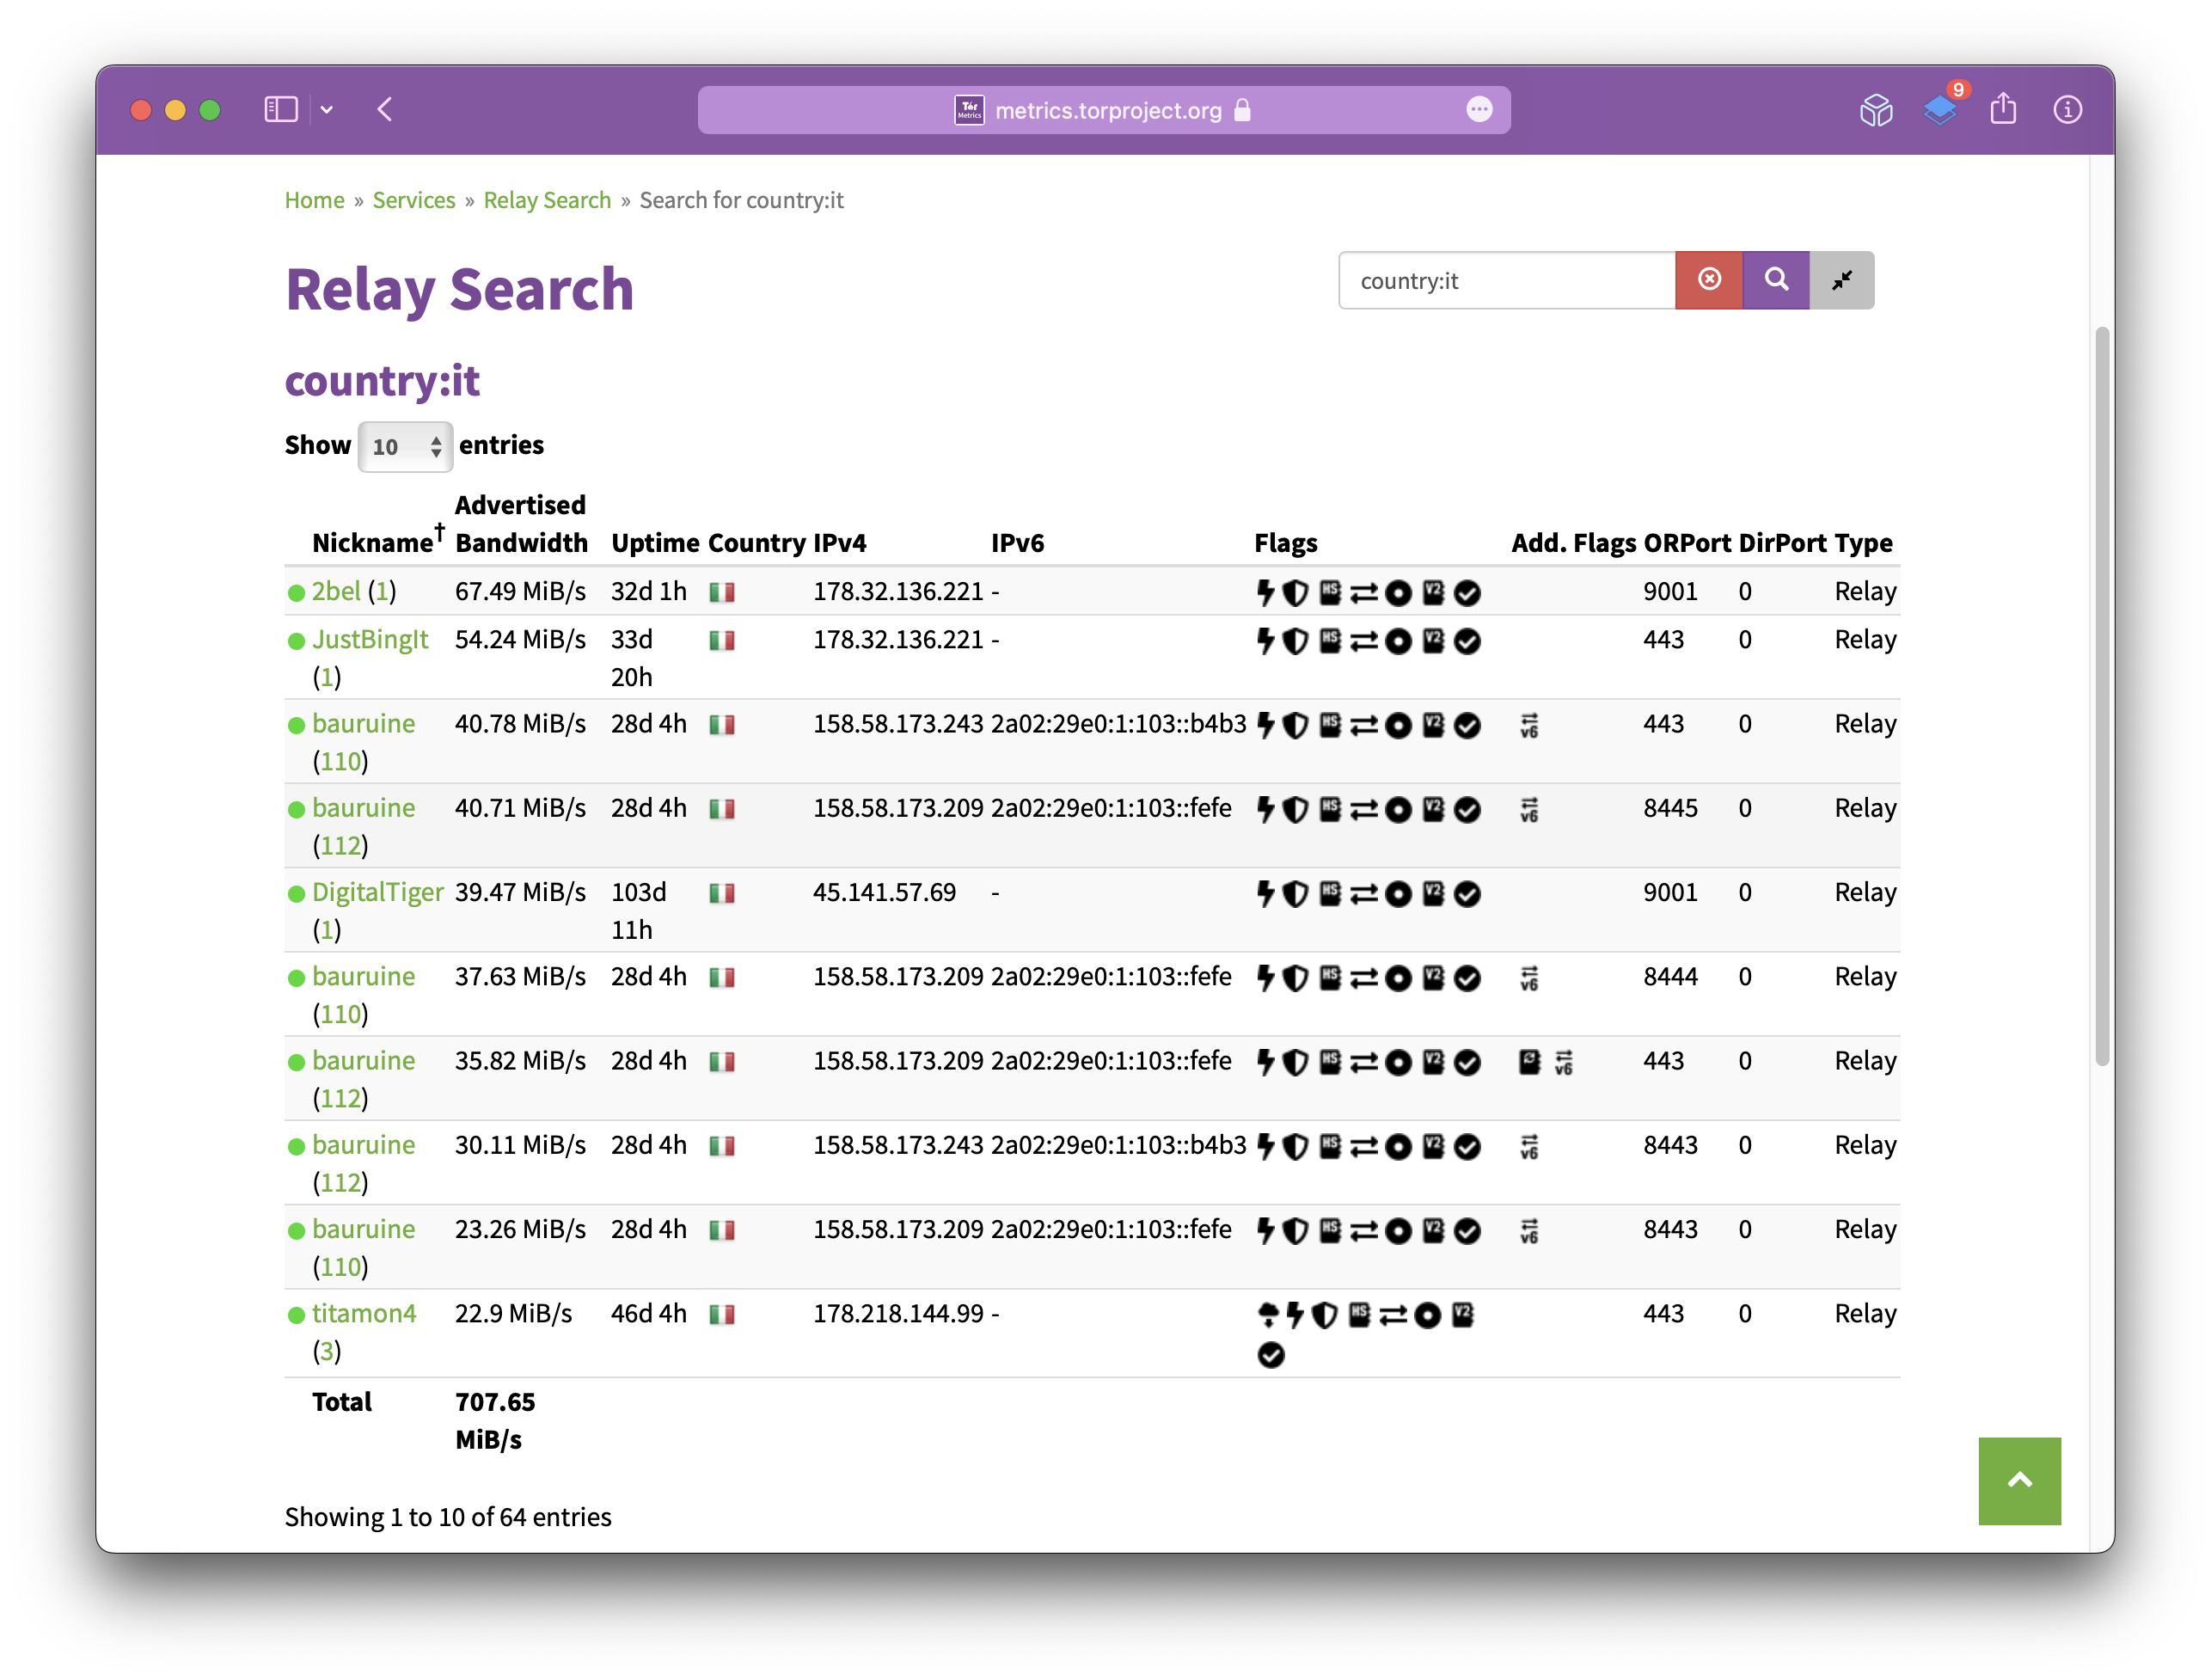
\includegraphics[width=\textwidth]{TorRelays}
    \caption{Statistiche dei Tor Relay in Italia}
}

\newpage
\section{Directory Servers} \label{sec:DirectoryServers}
I directory server sono un piccolo sottogruppo di onion router utilizzati per tracciare i cambiamenti nella topologia di rete. 
In particolare un directory server agisce come un server HTTP accessibile dai client per ottenere lo stato della rete e la lista dei router aggiornata periodicamente dagli stessi OR. \\
Quando il directory server riceve un aggiornamento da un OR prima di tutto controlla la chiave d'identità del router, garantendo che un attaccante non possa fingersi un OR manomettendo la rete \cite{ChaumMixes}. 
Il software di accesso alla rete onion è precaricato con le informazioni sui directory server e le relative chiavi, le informazioni di rete vengono aggiornate periodicamente dall'OP. \\

I directory server sono anche fondamentali per la connessione agli onion services, infatti ogni servizio creato genera un \emph{Onion Service Descriptor} contenente una lista degli introduction points e la chiave pubblica, il pacchetto viene criptato con la chiave privata e inviato al directory server che quindi agisce come fosse un DNS server per gli onion services. 
Quando l'utente tenta la connessione a un sito onion richiede e riceve dal directory server il relativo \emph{Descriptor} per l'indirizzo onion, usa la chiave pubblica, derivata dalla stringa dell'indirizzo onion a cui vuole connettersi, per decriptare il pacchetto \\
Nel caso il Directory Server fosse compromesso e contenesse un Descriptor malevolo generato per reindirizzare il traffico\footnote{Che però non potrà avere la stessa chiave privata}, l'indirizzo onion che possediamo non sarebbe in grado\footnote{tramite la chiave pubblica al suo interno nascosta} di decriptare le informazioni, dato che sono state criptate con una differente chiave privata
\cite{OnionServicesOverview}.
Non c'è neanche la necessità di determinare se le informazioni sono correte, perché a patto che la chiave privata non sia resa pubblica, nessuno potrà manomettere il Descriptor senza renderlo illeggibile e/o \emph{"indecifrabile"}
\section{Tor Browser}
Una delle principali vulnerabilità della rete Tor è la possibilità che un servizio web crei un codice JavaScript\footnote{che viene eseguito sul browser dell'utente} malevolo in grado di ottenere informazioni sull'indirizzo dell'utente deanonimizzandolo. 
Gli sviluppatori di Tor Browser hanno inserito appositamente un sistema di sicurezza che blocca gli script, questo però di contro porta molti siti a non funzionare correttamente. \\
Essendo la rete Tor fortemente basata sulla criptografia la navigazione di un sito onion tramite Tor non fa comparire alcun avviso di sicurezza in caso di mancanza di HTTPS, dato che il traffico è già criptato. 
Da tenere inoltre in considerazione che un certificato proveniente da una Certificate Authority potrebbe generare problemi di anonimizzazione del servizio a causa della Certificate Transparency\cite{CertificateTransparency} \\
\newpage
\section{Dimostrazione da Wireshark}

Ci sono diversi elementi che possono indicare l'esistenza di un circuito onion, innanzitutto esso viene creato sfruttando il protocollo TLS\footnote{In particolare la nuova versione di Tor usa TLSv1.3} tramite TCP, inserendo quindi TLS come filtro in Wireshark possiamo vedere i pacchetti con cui viene generato il circuito.
\importImage{
    \label{fig:Wireshark_circuit_raw}
    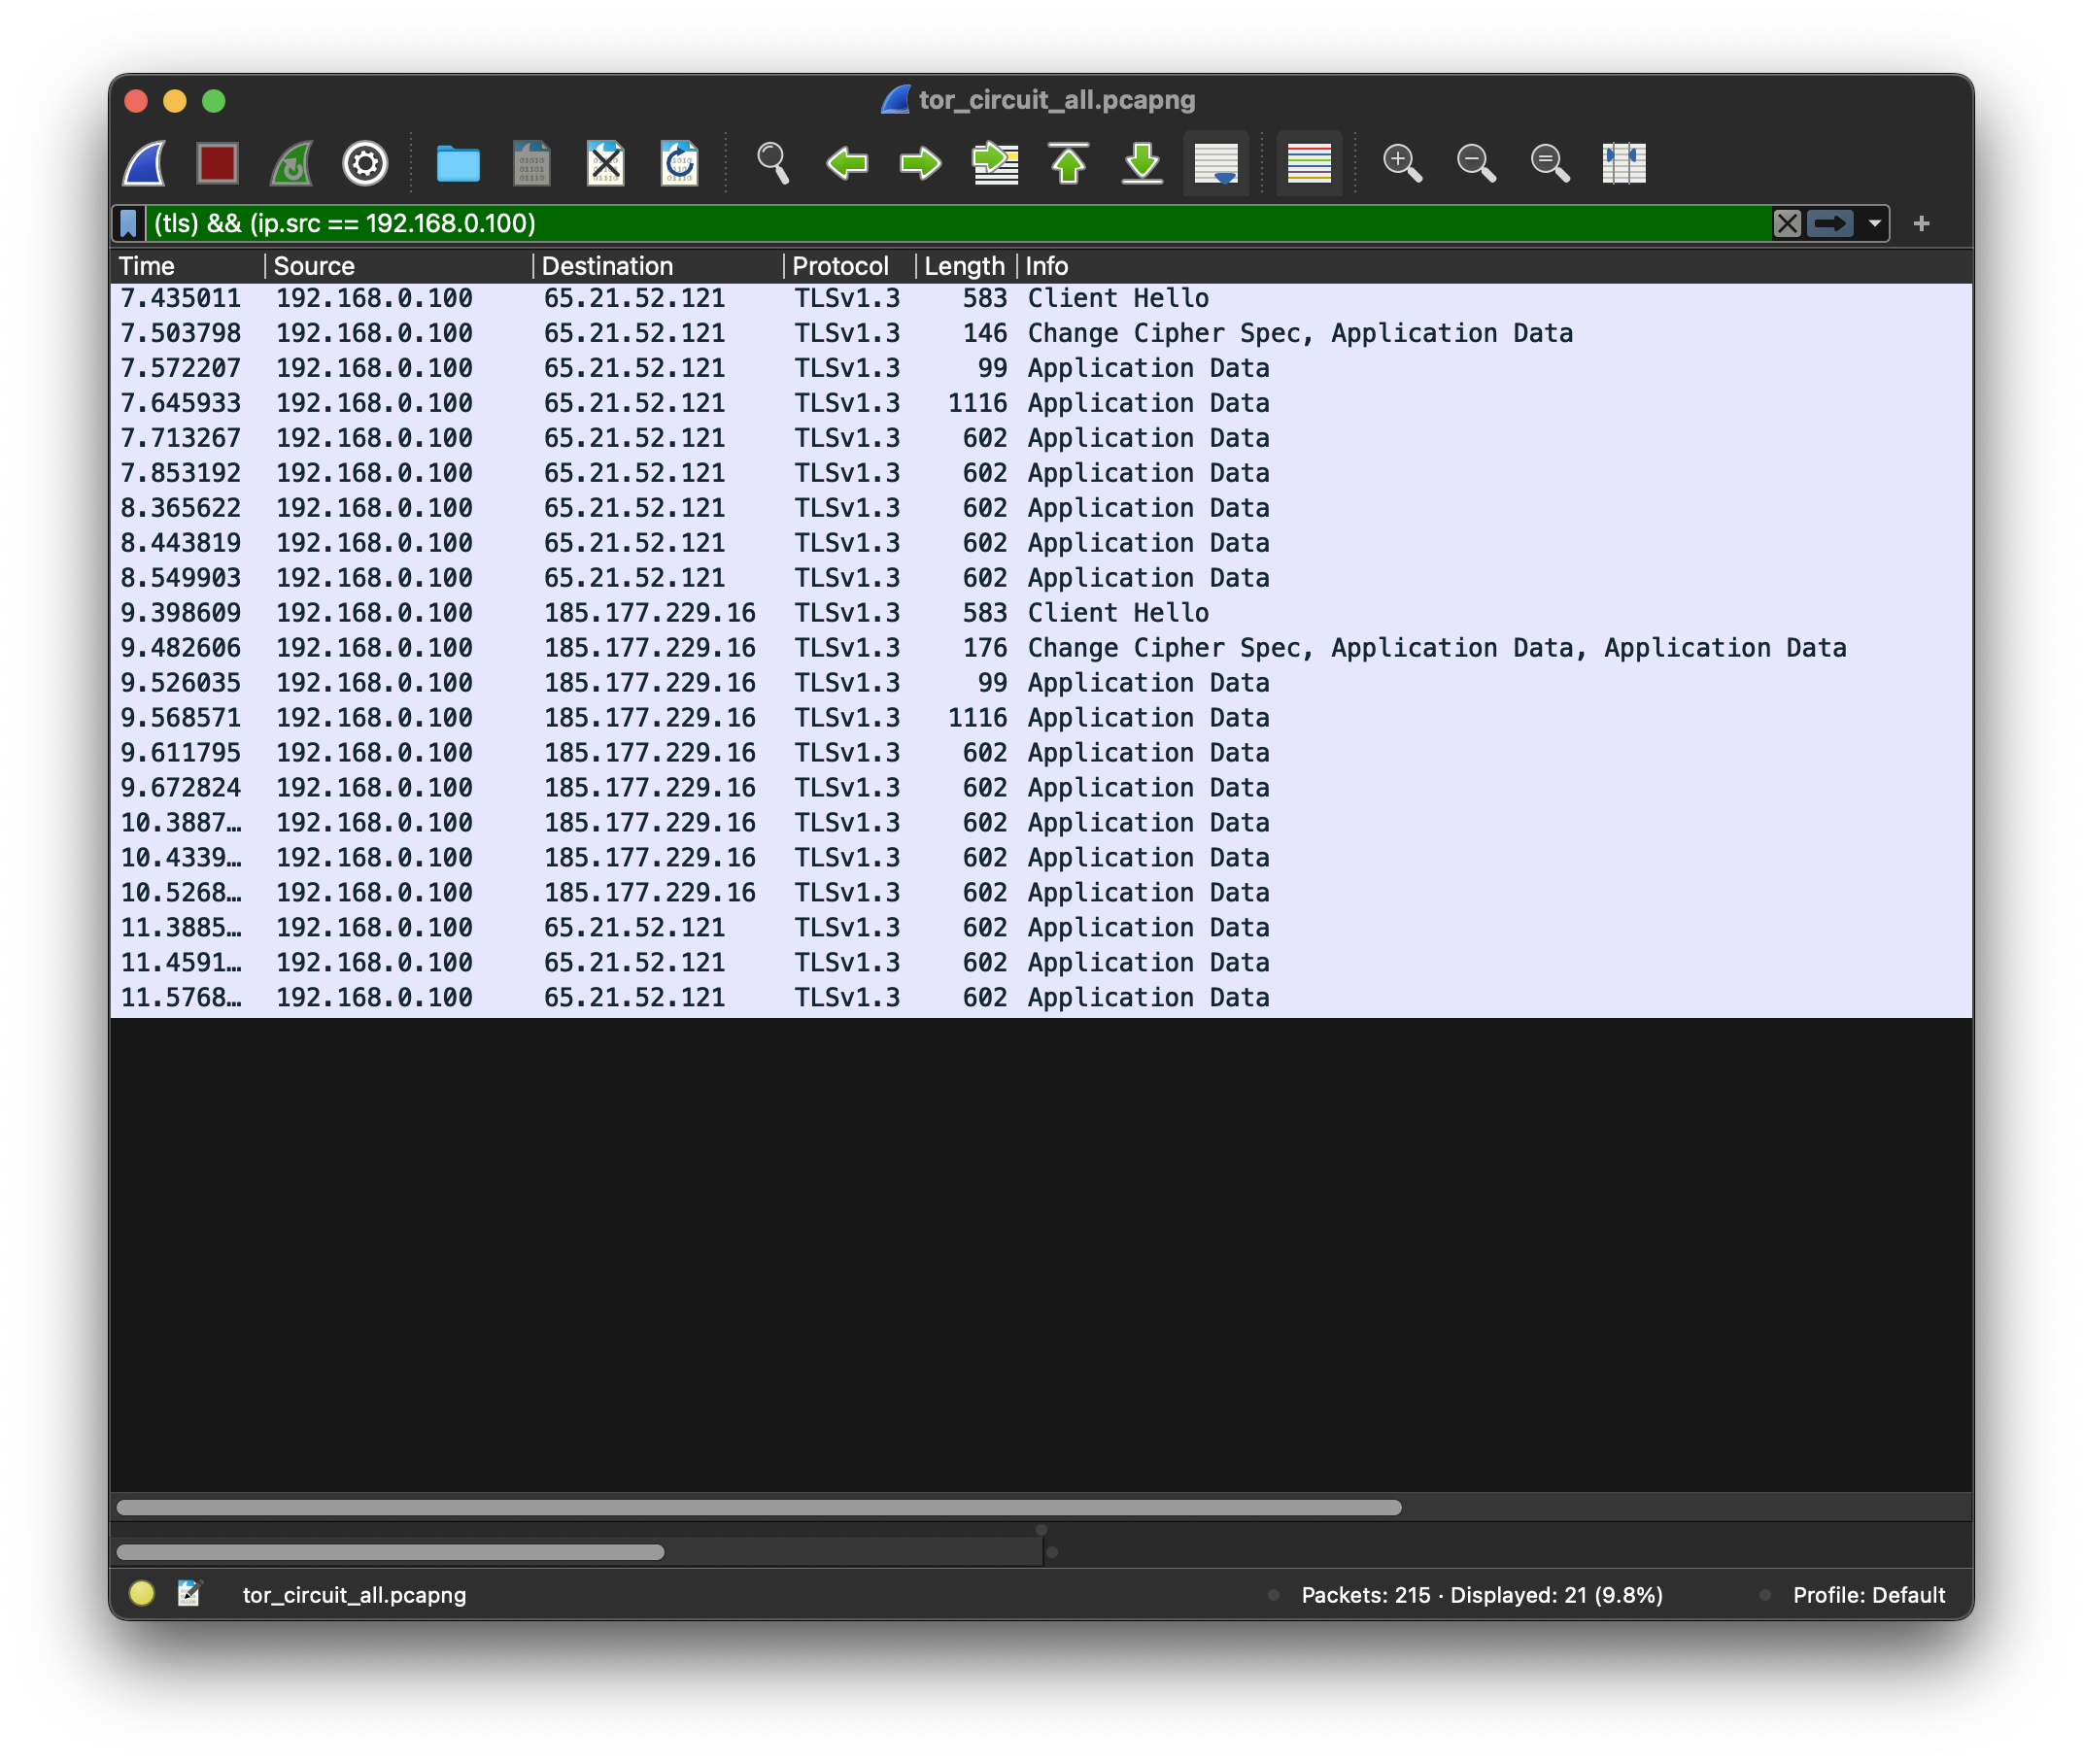
\includegraphics[width=\textwidth]{Wireshark/circuit_raw}
    \caption{Wireshark circuit}
}\\
Da qui vediamo che i due IP principali a cui il dispositivo si connette sono \lstinline{65.21.52.121} e \lstinline{185.177.229.16}. Vediamo anche che Tor scambia con questi due IP lo stesso numero e tipo di pacchetti con la stessa quantità di byte, per cui vi è una correlazione.
Eseguendo il filtro per IP possiamo quindi vedere tutti i pacchetti che i due dispositivi si scambiano
\newpage
\importImage{
    \label{fig:Wireshark_IP_Filtering}
    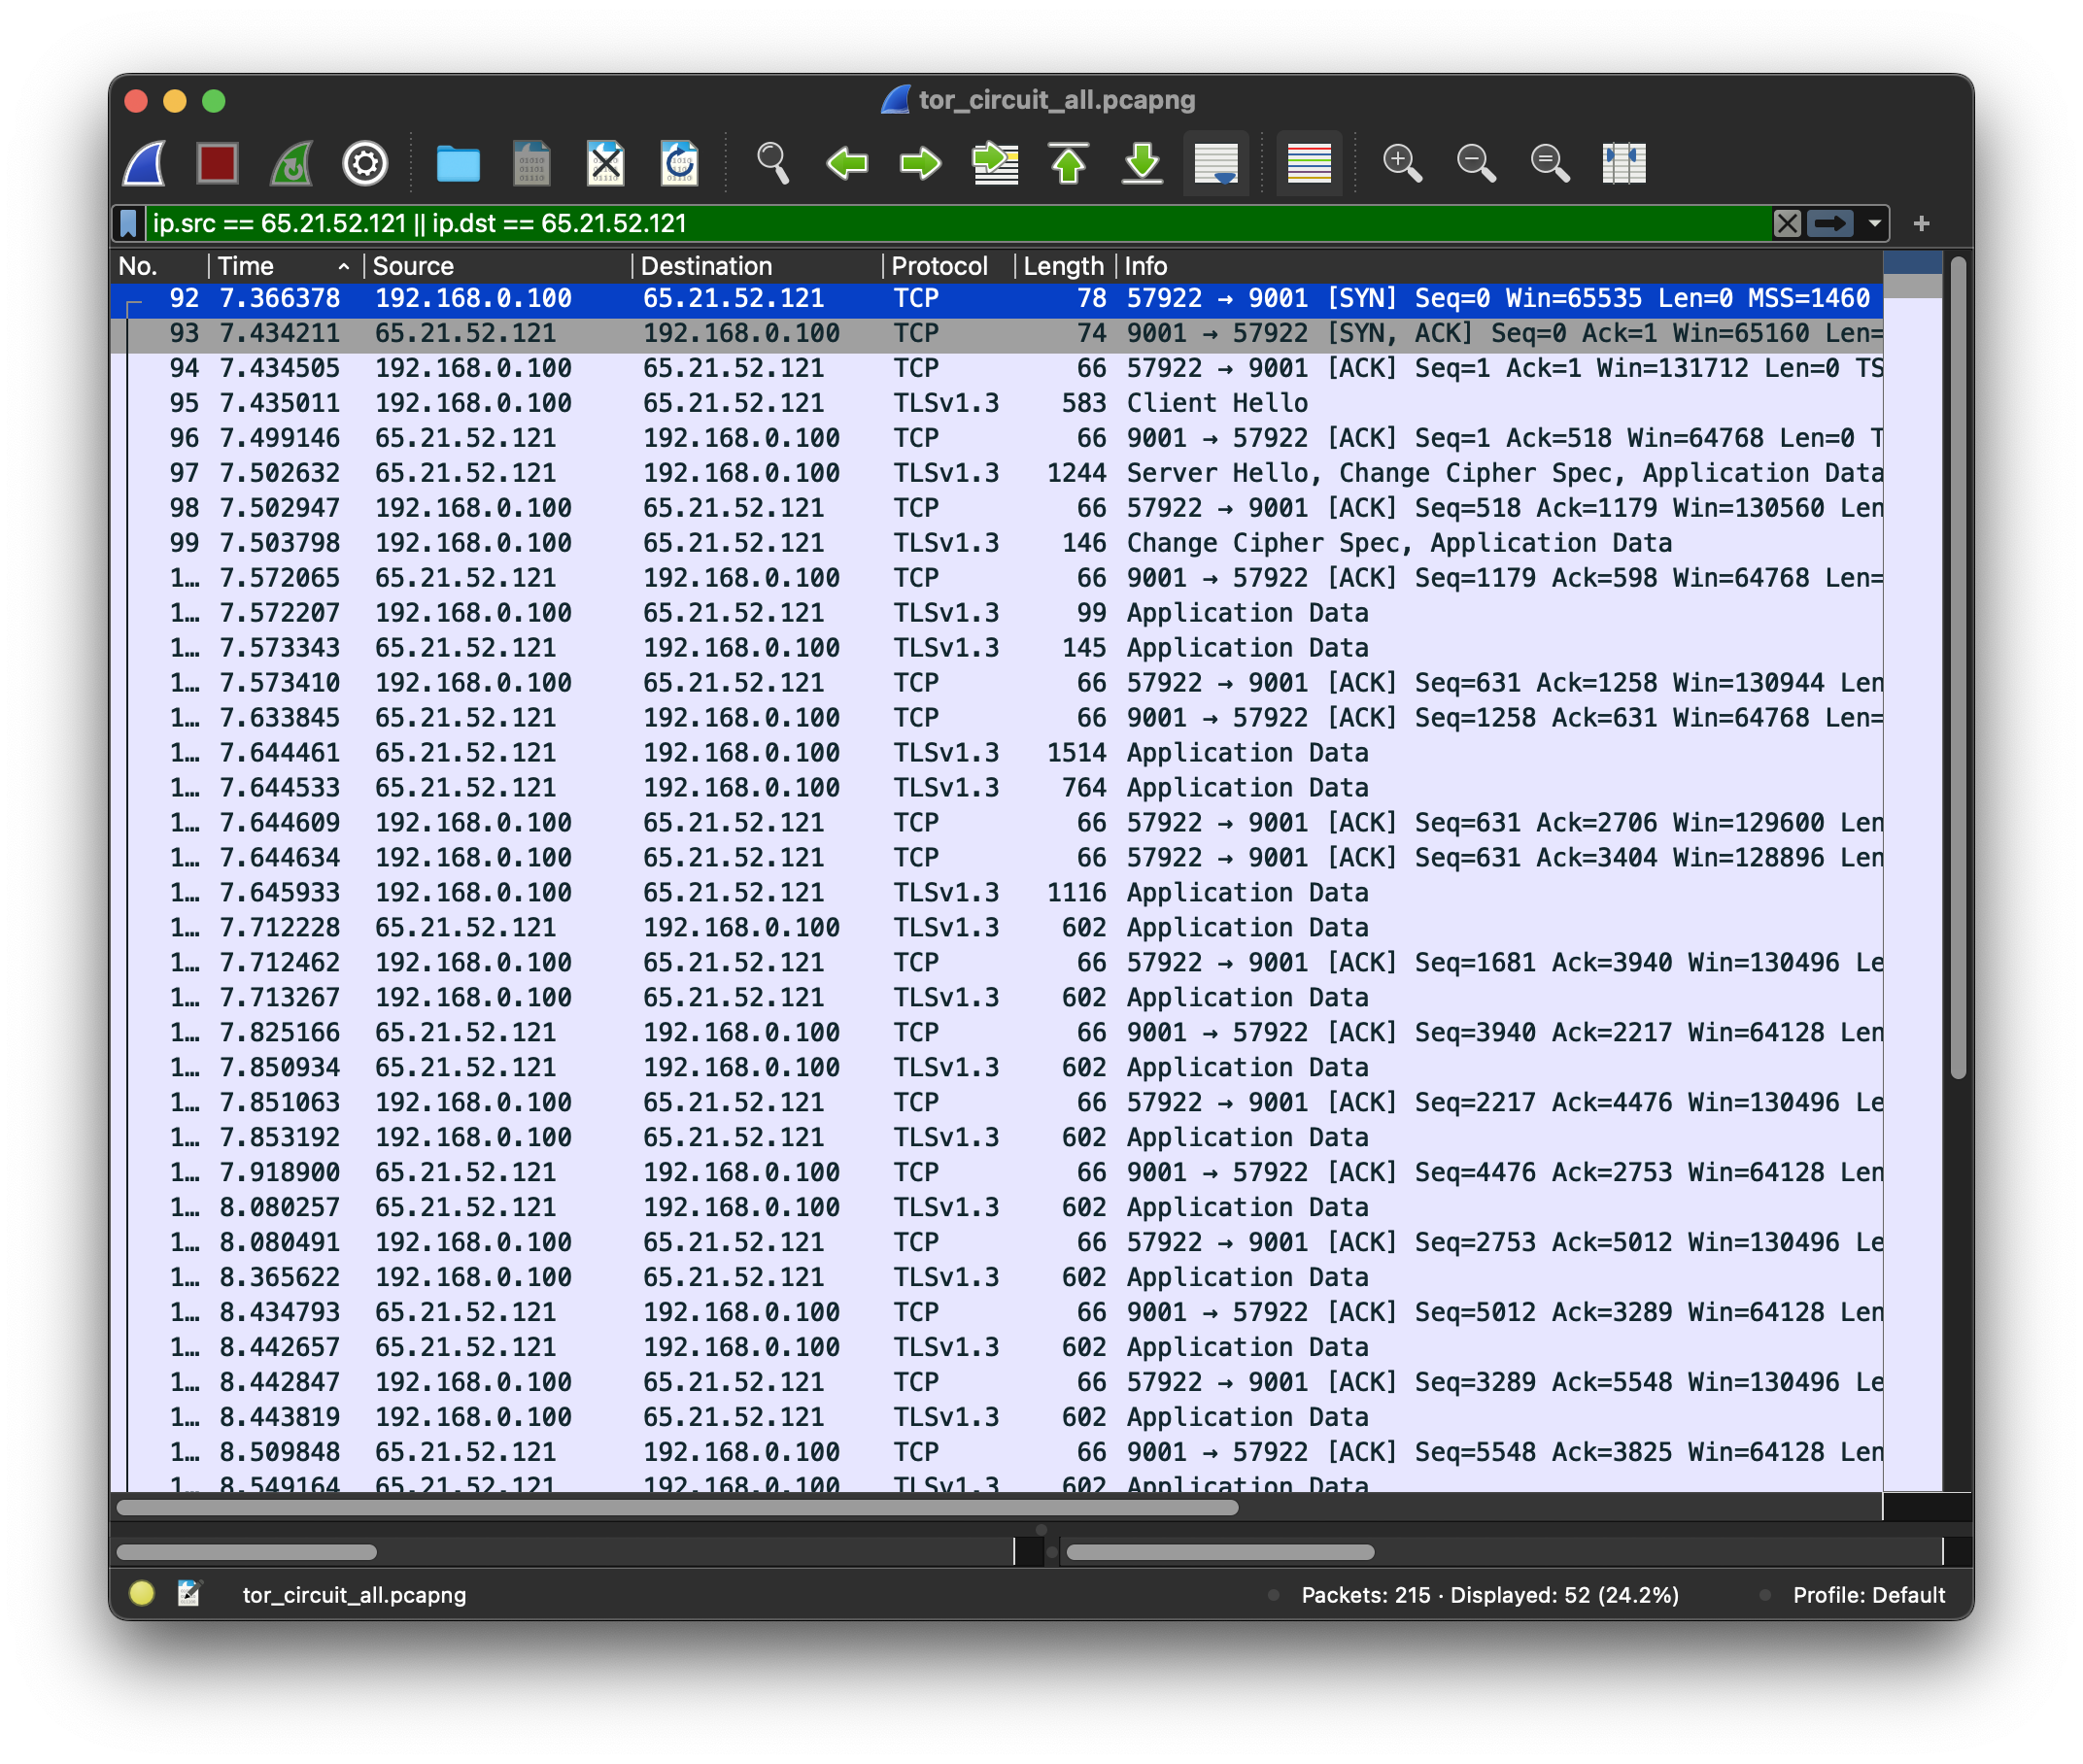
\includegraphics[width=\textwidth]{Wireshark/IP_Filtering}
    \caption{Wireshark IP filtering}
}
Vediamo quindi che inizialmente viene eseguito un TCP handshake, successivamente inizia lo scambio di chiavi tramite TLSv1.3, possiamo inoltre notare che la porta con cui comunichiamo con il server \lstinline{65.21.52.121} è la 9001\footnote{Tor Project suggerisce di non usare la porta 9001 per i bridge relay perché è facilmente associabile alla rete Onion\cite{OnionAvoid9001}}.
A ogni messaggio TLS corrisponde una risposta ACK TCP che possiamo ignorare.
\newpage
Analizziamo il primo pacchetto TLS che viene inviato al server, è denominato \textbf{Client Hello} e possiede vari campi
\begin{itemize}
    \item \textbf{Cipher Suites}, una lista di protocolli di criptografia simmetrica supportati dal client che invia la richiesta\cite{RFC8448}. In questo caso i protocolli supportati sono 18, tra cui abbiamo \lstinline{AES 128 GCM SHA256} e \lstinline{AES 256 GCM SHA384}
    \item Compression Methods, implementato in TLSv1.3 solo per retro compatibilità dei server, che possono anche ricevere e gestire richieste TLSv1.2. A differenza dei client TLSv1.3 che devono impostare questo parametro a 0 (null), altrimenti riceveranno un \lstinline{illegal_parameter message}
    \item \textbf{Extensions}, usato sia dalle applicazioni che sfruttano TLS, come onion, che da alcune funzionalità di TLSv1.3, implementate come estensioni per mantenere la retro compatibilità. In tal modo i server legacy possono semplicemente ignorare le estensioni non riconosciute
\end{itemize}
\cite{TLSv1_3}
\importImage{
    \label{fig:Client_Hello}
    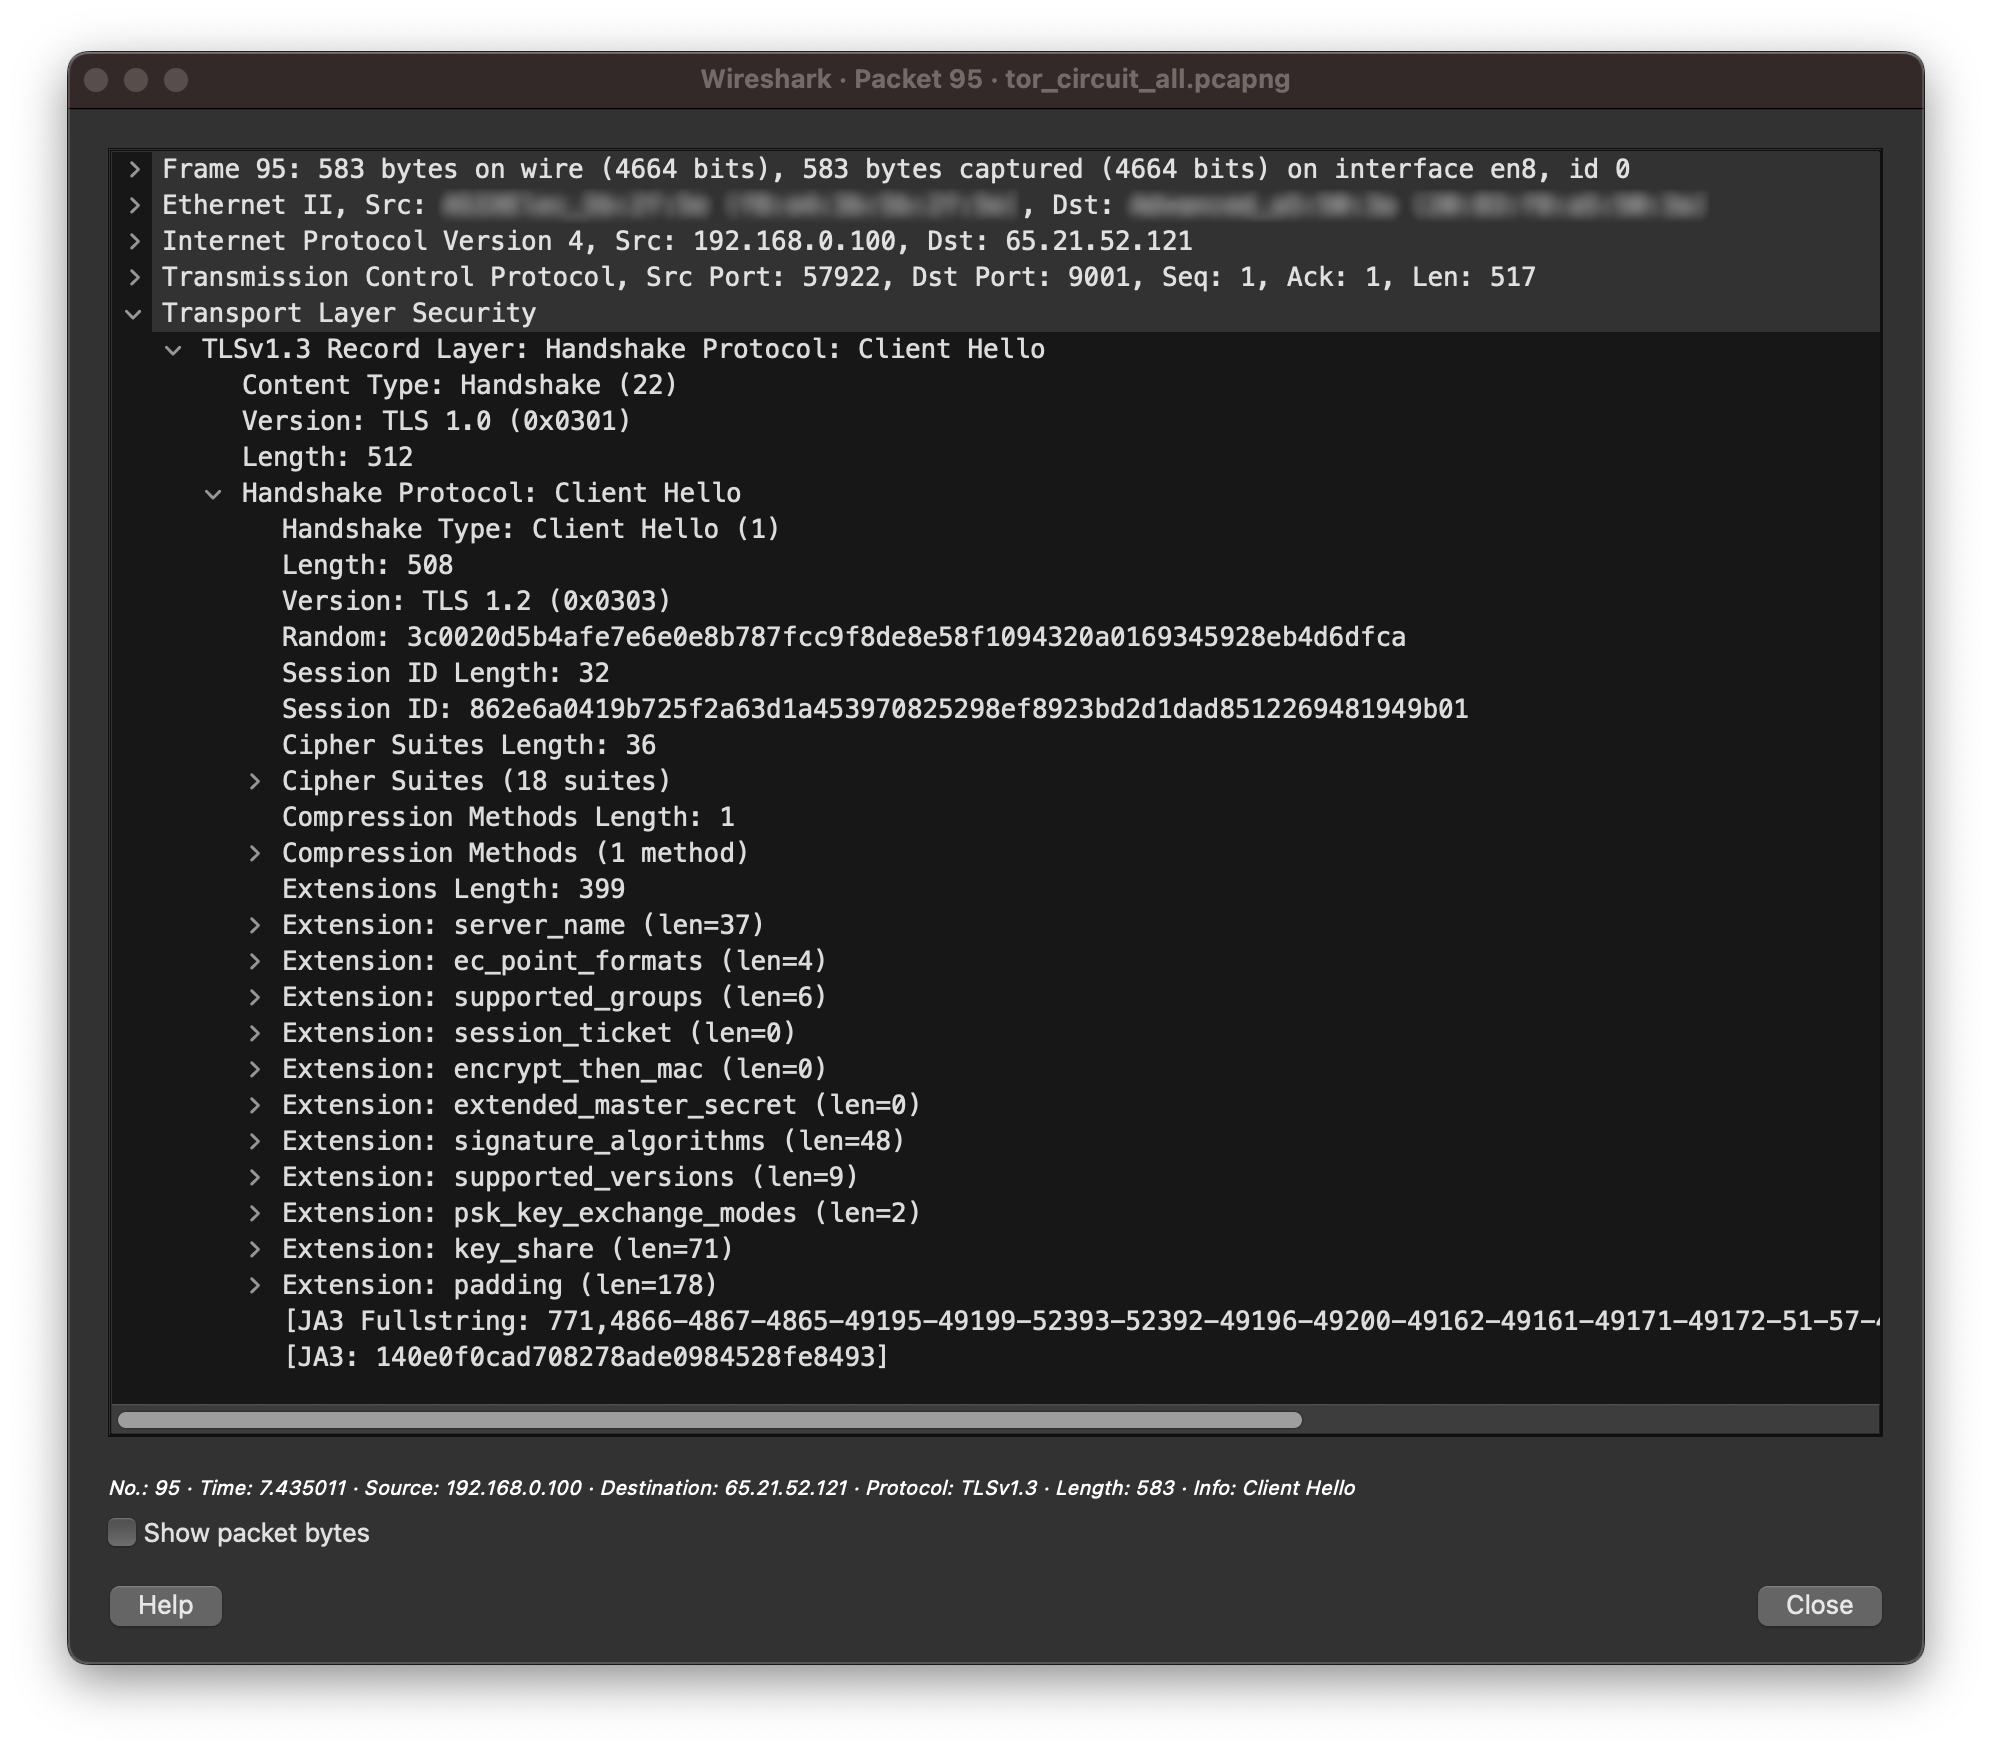
\includegraphics[width=\textwidth]{Wireshark/Client_Hello}
    \caption{Client Hello}
}
\newpage
Come vediamo onion sfrutta diverse estensioni
\begin{itemize}
    \item \lstinline{server_name}, utilizzato per facilitare le connessioni sicure, indica il nome del server\cite{RFC6066}
    \item \lstinline{ec_point_formats}, sta per Elliptic Curve Point Formats e indica i formati di compressione(Point Formats) supportati dal client\cite{RFC8422}
    \item \lstinline{supported_groups}, precedentemente chiamato Supported Elliptic Curves Extensions, indica gli Elliptic Curves utilizzati ordinati in base alla preferenza del client \cite{RFC8422}
    \item \lstinline{session_ticket}, non usato
    \item \lstinline{encrypt_then_mac}, non usato
    \item \lstinline{extended_master_secret}, non viene più usato ma deve comunque essere indicato per retro compatibilità\cite{RFC7627}
    \item \lstinline{signature_algorithms}, utilizzato per indicare gli algoritmi di firma supportati dal client\cite{RFC8446}
    \item \lstinline{supported_versions}, utilizzato dal client per indicare le versioni di TLS supportate e dal server per indicare la versione utilizzata \cite{RFC8446}
    \item \lstinline{psk_key_exchange_modes}, utilizzato esclusivamente dal client per indicare le modalità di condivisione della passkey\cite{RFC8446}
    \item \lstinline{key_share}, utilizzato per inviare la chiave pubblica con cui criptare il traffico del server verso questo client, indicando anche il tipo di chiave\cite{RFC8446}
    \item \lstinline{padding}, utilizzato come una sequenza di 0 sufficienti per far raggiungere al pacchetto almeno 512 bytes di lunghezza. Il campo può essere omesso per i pacchetti di almeno 512 bytes. Con pacchetti di lunghezza tra 509 e 511 bytes questo campo porta il pacchetto a superare i 512 bytes, in quanto non può essere inferiore ai 4 bytes\cite{RFC7685}
\end{itemize}
\newpage
Successivamente il server risponde con un \textbf{Server Hello}, indicando un unico cipher suite e le estensioni \lstinline{supported_versions} e \lstinline{key_share}.
\importImage{
    \label{fig:Server_Hello}
    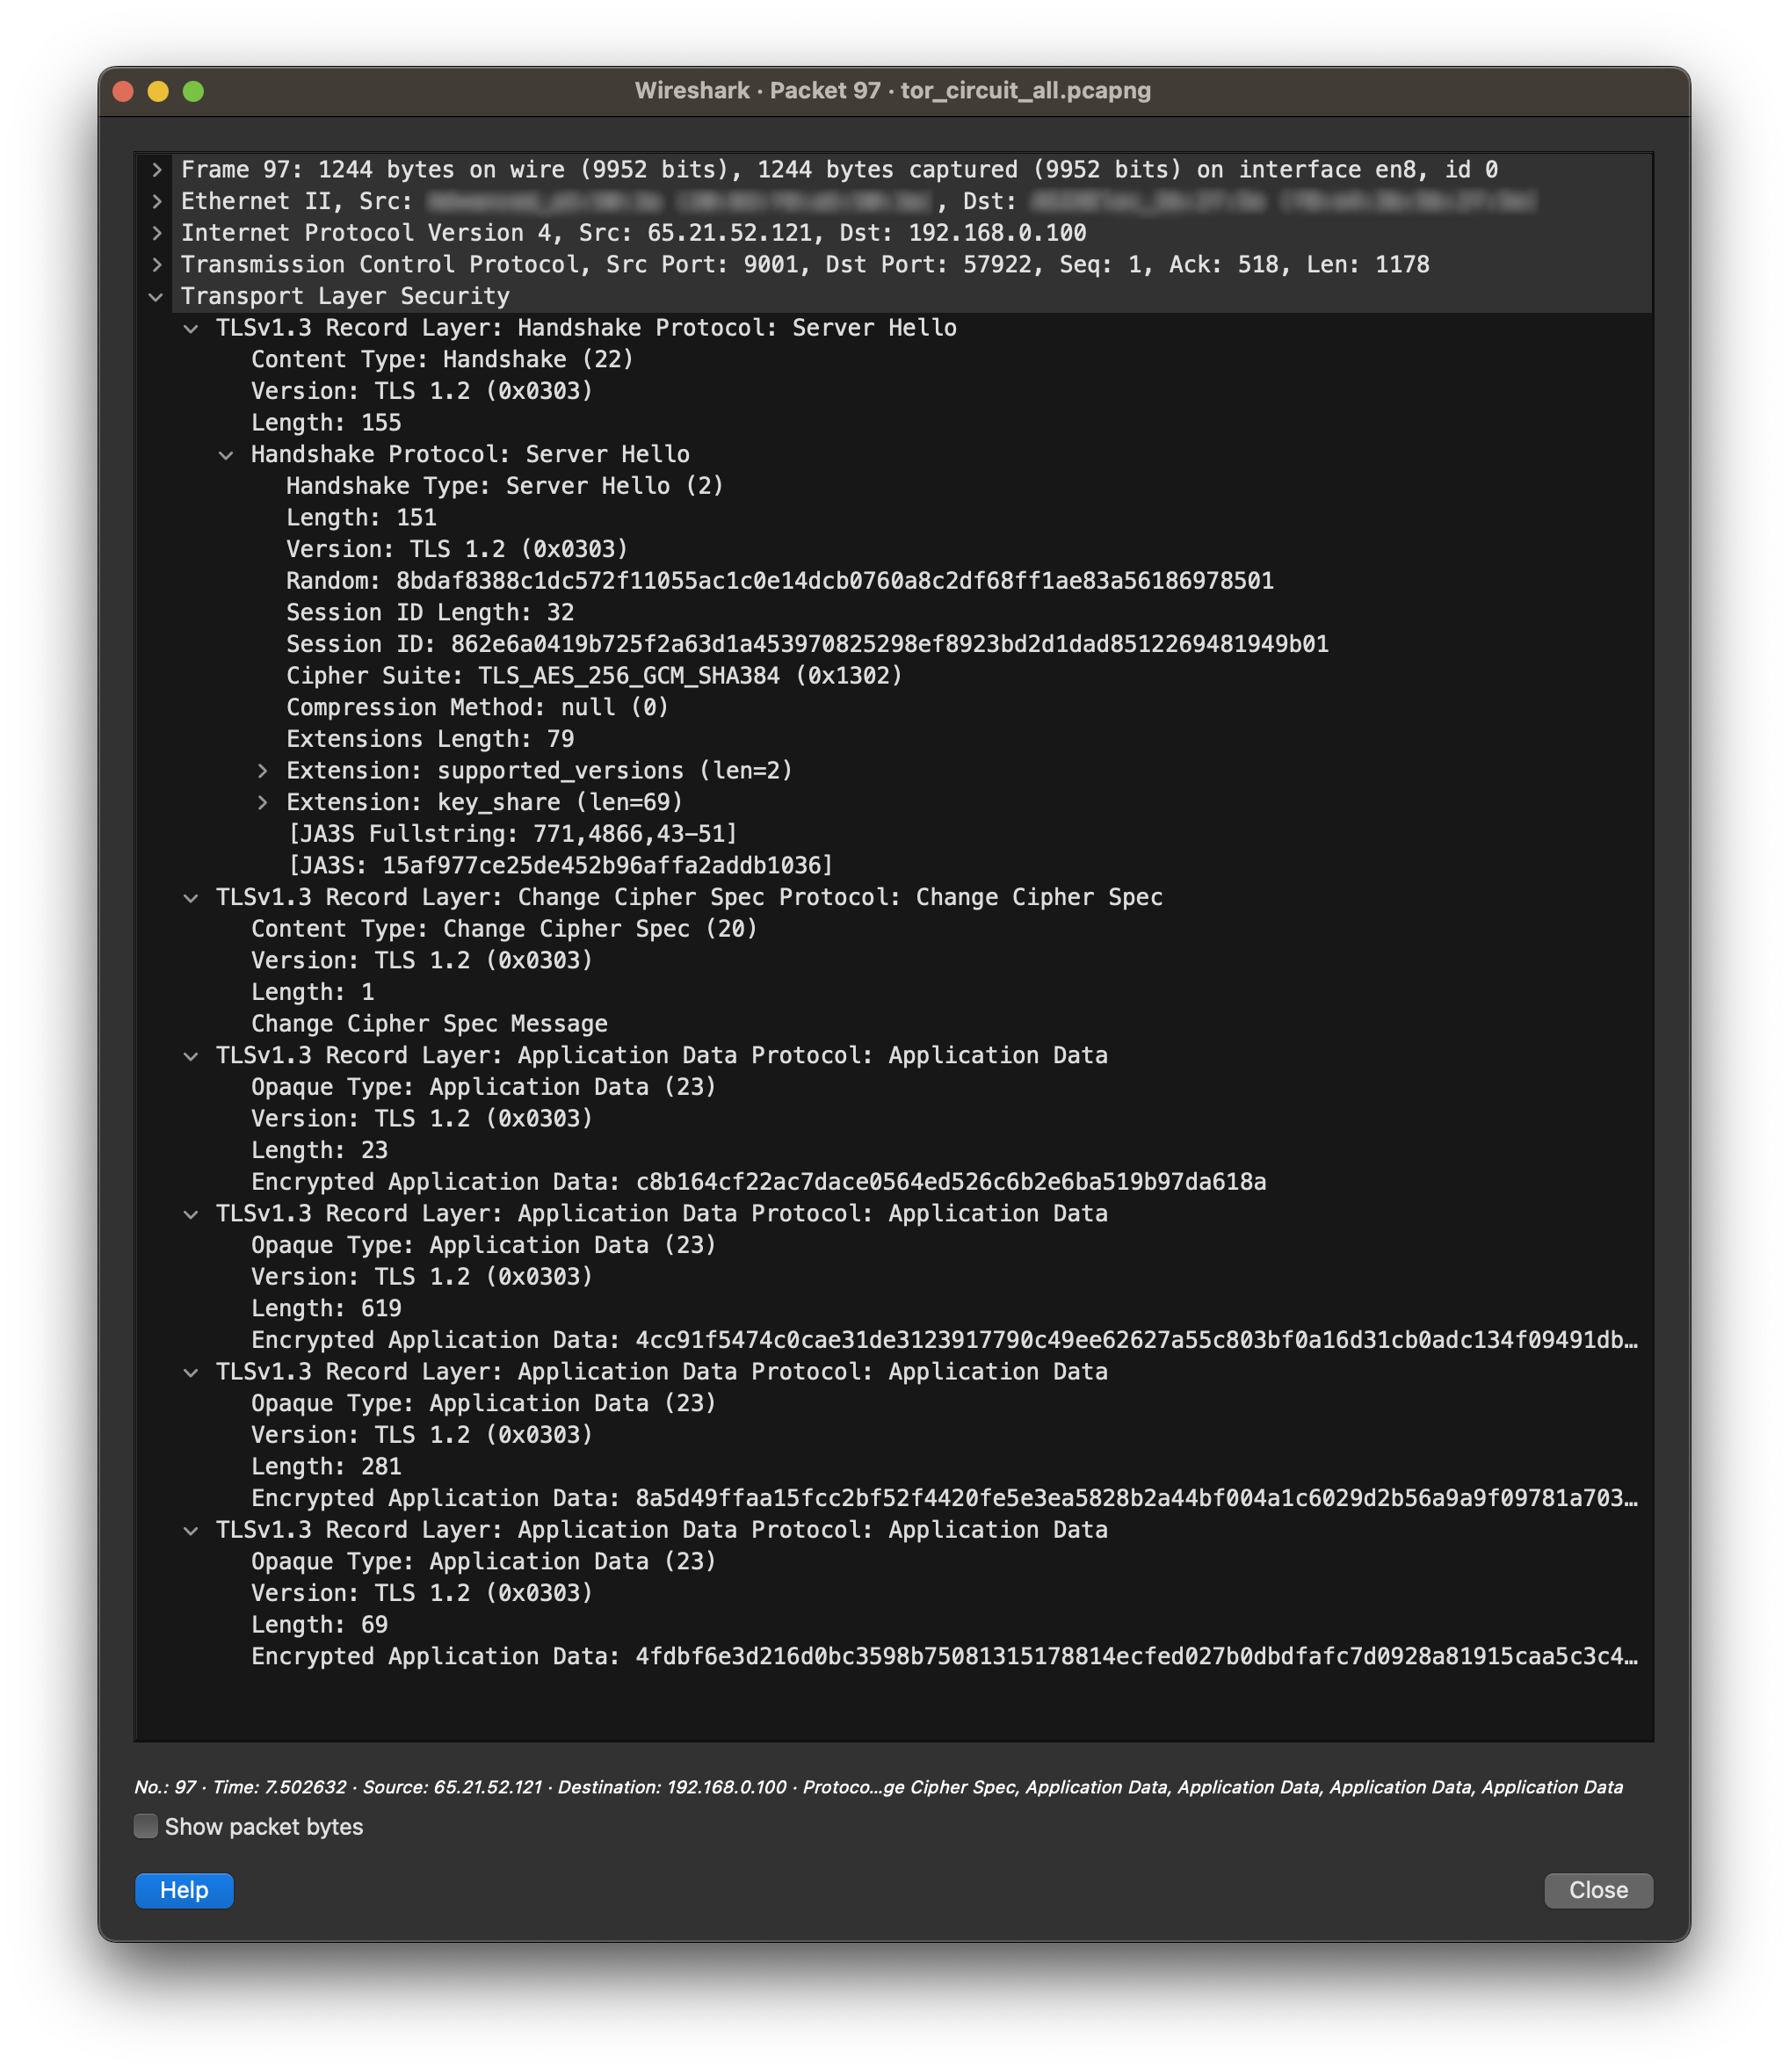
\includegraphics[width=\textwidth]{Wireshark/Server_Hello}
    \caption{Server Hello e Application Data}
}\\
Da qui la connessione viaggia per il circuito onion e tutti i dati sono criptati con le chiavi che possiede solo il client Tor, per cui non è possibile analizzare il traffico, possiamo solo intuire quali pacchetti sono destinati alla rete onion.


% \section{Vulnerabilità} % Qui si parla delle vulnerabilità di onion v2 per cui si è passati a v3

\section{Implementazione}
\begin{frame}{Implementazione}
    Per implementare un servizio onion è necessario utilizzare un \textbf{Proxy Onion} per inoltrare le richieste dalla rete Tor al server web. Il proxy gestisce la generazione delle chiavi, dell'indirizzo e la definizione e connessione con gli \textbf{introduction points}, oltre alla generazione del descriptor e la sua pubblicazione nei Directory Servers. \\
    In particolare la nostra implementazione \textbf{Onion V3} (dato che Onion V2 è stato deprecato) userà un server \textbf{Linux} su AWS per ospitare il Proxy Onion e un \textbf{server nginx}.
\end{frame}

\begin{frame}
    Nel sistema è necessario installare il web server NGINX e dopo una serie di configurazioni dei repository possiamo installare il Proxy Tor. Nel file di configurazione \hyperref[torConfig]{torrc} è possibile indicare la directory in cui salvare le chiavi e il tipo di connessione con il web server. \\
    In questa implementazione ho usato un tool (\href{https://github.com/cathugger/mkp224o/}{mkp224o}) per generare la coppia chiave privata e pubblica che risulti in un indirizzo onion personalizzato.
\end{frame}

\begin{frame}
    \centering
    \href{http://tesilm3jb64lw3upj4uu5fsxi2nrtbhbhkbu2dsbn46qka7j4kf7peqd.onion}{http://tesilm3jb64lw3upj4uu5fsxi2nrtbhbhk bu2dsbn46qka7j4kf7peqd.onion}
    \begin{figure}
        \centering
        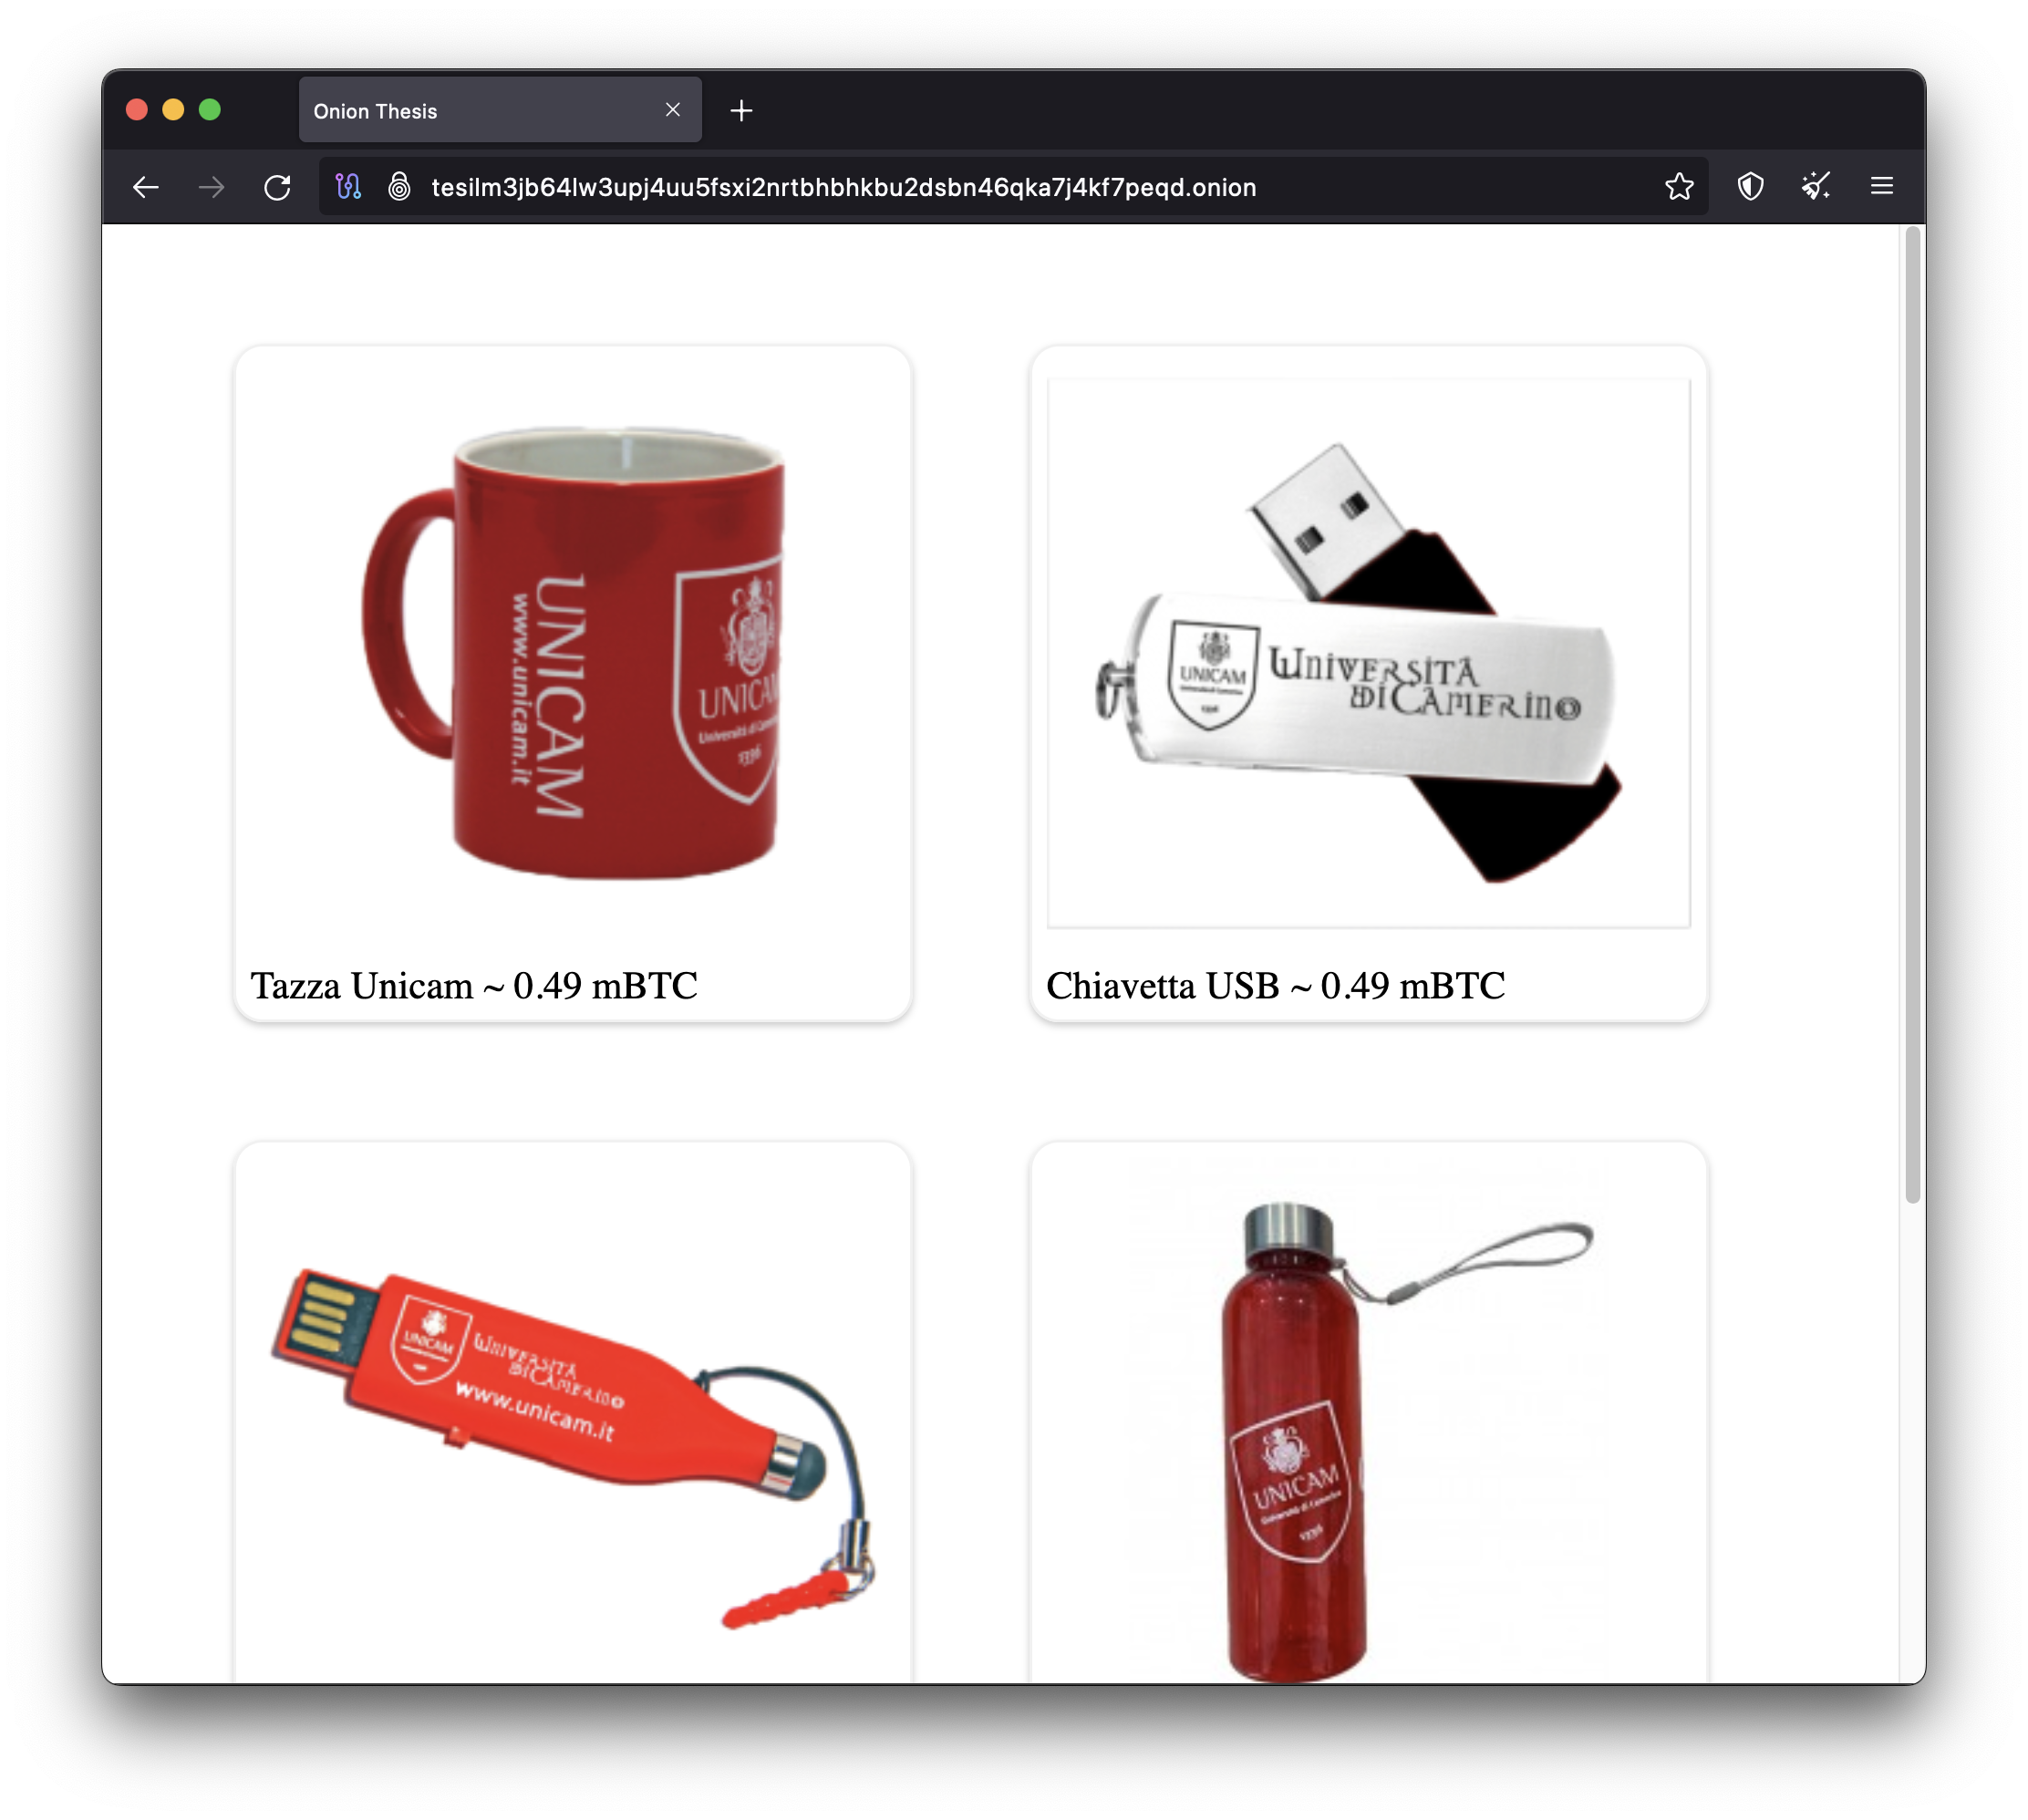
\includegraphics[width=0.8\textwidth]{OnionConnection.png}
    \end{figure}
\end{frame}

\subsection{Pubblicizzare il servizio}
\begin{frame}{Pubblicizzare il servizio}
    Nel lavoro di tesi abbiamo mostrato come pubblicizzare il servizio onion tramite un'\textbf{Header Tag}, è infatti possibile inserire un tag all'interno della pagina html che quando aperto con Tor consente di reindirizzare l'utente al relativo sito onion.
    \href{http://tesilm3jb64lw3upj4uu5fsxi2nrtbhbhkbu2dsbn46qka7j4kf7peqd.onion}{\lstinline{<meta http-equiv="onion-location" content="http://tesilm3jb64lw3upj4uu5fsxi2nrtbhbhkbu2dsbn46qka7j4 kf7peqd.onion" />}}
    % The space is important to make the line break correctly
\end{frame}

\begin{frame}
    \begin{figure}
        \centering
        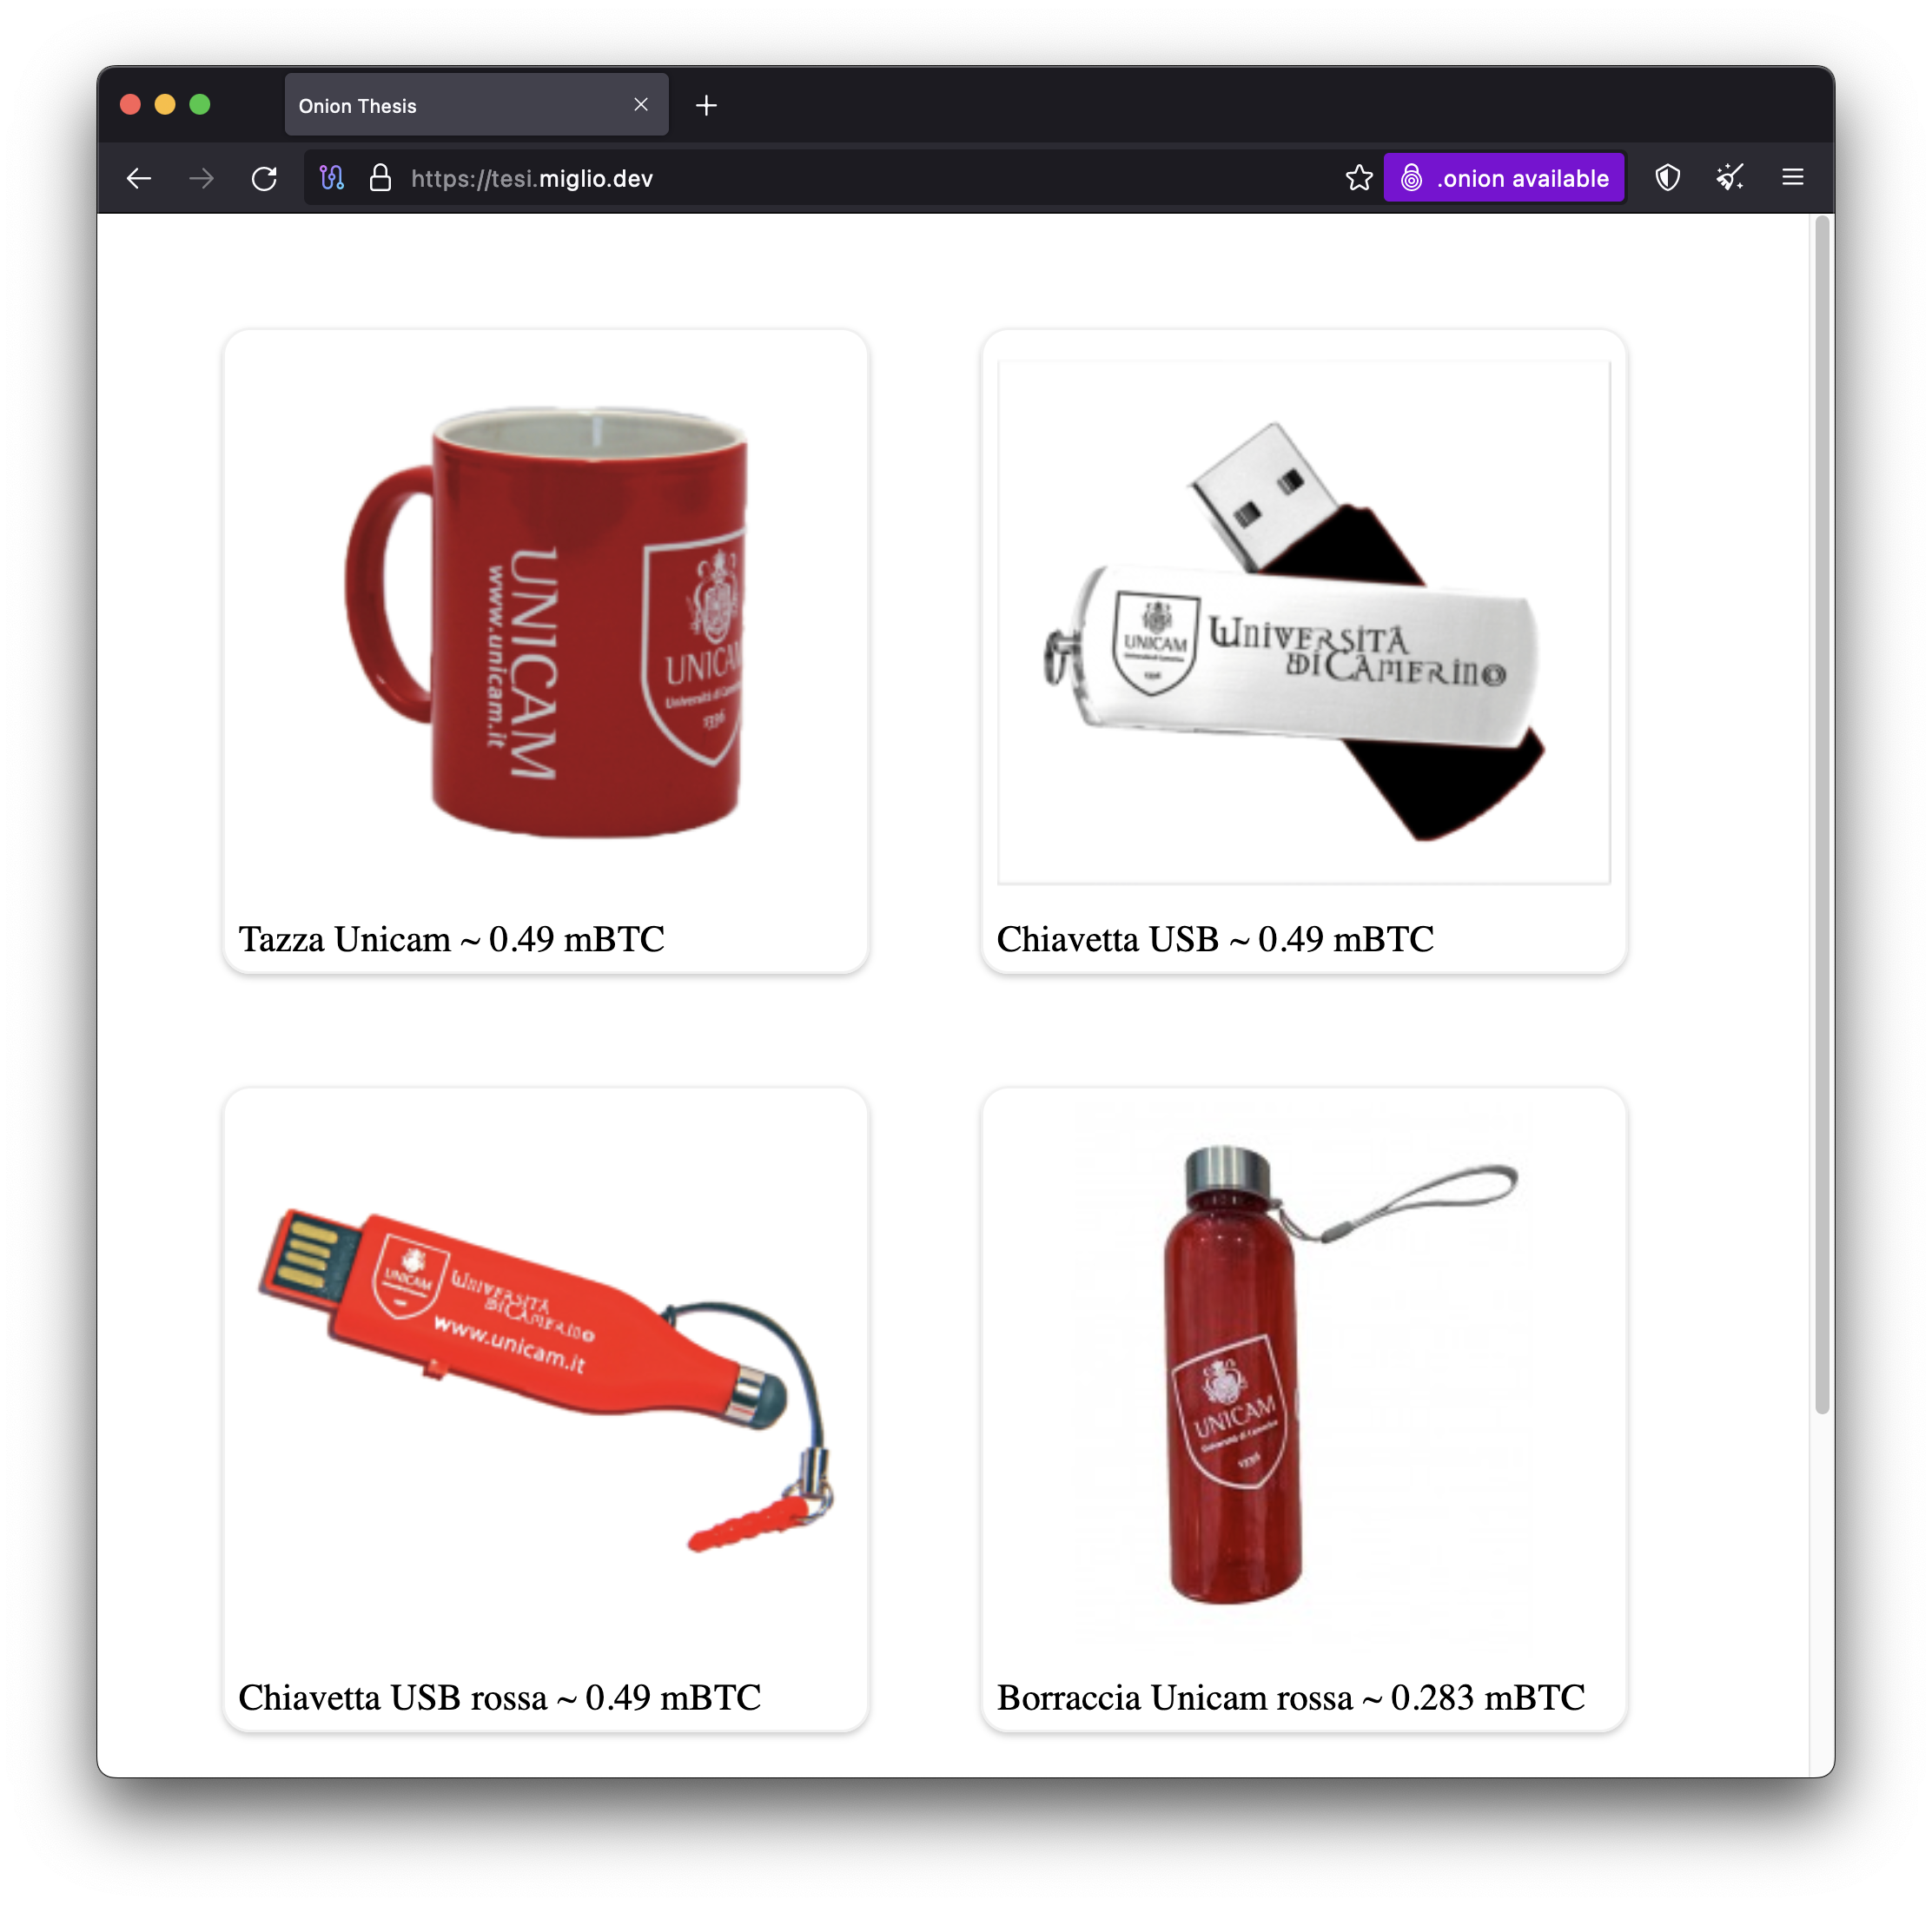
\includegraphics[width=0.8\textwidth]{ClearWebPage}
    \end{figure}
\end{frame}



%%%%%%%%%%%%%%%%%%%%%%%%%%%%%%%%%%%%%%%%%%%%%%%%%%%%%%

\end{document}
% TODO completa cap 5